\documentclass[12pt]{report}
\usepackage[utf8]{inputenc}
\usepackage[spanish]{babel}
\usepackage{graphicx}
\usepackage{pifont}
\usepackage{url}
\usepackage{listings}
\usepackage{color}
\usepackage{chngcntr}
\usepackage{caption}
\usepackage{parskip}
\usepackage{titlesec} 
\usepackage[nottoc]{tocbibind}
\usepackage[backend=biber,safeinputenc,sorting=none]{biblatex}
\usepackage[nodayofweek]{datetime}
\usepackage{hyperref}
\usepackage{minted}
\usemintedstyle{colorful}
\bibliography{references}

\setlength\bibitemsep{0.5\baselineskip}

\definecolor{lightgray}{rgb}{.9,.9,.9}
\definecolor{darkgray}{rgb}{.4,.4,.4}
\definecolor{purple}{rgb}{0.65, 0.12, 0.82}

\lstdefinelanguage{JavaScript}{
  keywords={typeof, new, true, false, catch, function, return, null, catch, switch, var, if, in, while, do, else, case, break},
  keywordstyle=\color{blue}\bfseries,
  ndkeywords={class, export, boolean, throw, implements, import, this},
  ndkeywordstyle=\color{darkgray}\bfseries,
  identifierstyle=\color{black},
  sensitive=false,
  comment=[l]{//},
  morecomment=[s]{/*}{*/},
  commentstyle=\color{purple}\ttfamily,
  stringstyle=\color{blue}\ttfamily,
  morestring=[b]',
  morestring=[b]"
}

\lstset{
   language=JavaScript,
   extendedchars=true,
   basicstyle=\footnotesize\ttfamily,
   showstringspaces=false,
   showspaces=false,
   tabsize=2,
   breaklines=true,
   showtabs=false,
   captionpos=b
}

\newdateformat{mydate}{\shortmonthname[\THEMONTH], \THEYEAR}

\counterwithout{footnote}{chapter}
\renewcommand*{\thefootnote}{\arabic{footnote}}
\graphicspath{ {images/} }
\title{
	{Desarrollo de un editor de visualizaciones de propiedades de historiales de wikis}\\
	{\large Universidad Central de Venezuela}\\
}
\author{Leonardo Testa}

\begin{document}

\begin{titlepage}
	\centering
  {\large República Bolivariana de Venezuela \par}
  {\large Universidad Central de Venezuela\par}
  {\large Facultad de Ciencias\par}
  {\large Escuela de Computación\par}\vspace{2cm}

	
\includegraphics[scale=0.60]{ucv_logo.png}\par\vspace{1cm}
	{\scshape\Large\textbf{Desarrollo de un editor de visualizaciones de propiedades de historiales de wikis}\par}
	\vfill

  	{\large Trabajo Especial de Grado presentado ante la ilustre Universidad Central de Venezuela por el Br. Leonardo Testa para optar al título de Licenciado en Computación.\par}
    {\large Tutor Prof. Eugenio Scalise \par}
	{\large \mydate\today \par}
\end{titlepage}

% Resumen
\chapter*{Resumen}
\textbf{Título:}\\
Desarrollo de un editor de visualizaciones de propiedades de historiales de wikis.

\textbf{Autor:}\\
Leonardo Testa.

\textbf{Tutor:}\\
Prof. Eugenio Scalise.

Un Wiki es un sitio web, generalmente de carácter informativo (como lo es Wikipedia), que puede ser modificado por múltiples personas. Cada una de estas modificaciones son almacenadas, y en conjunto conforman un historial de versiones, en donde cada versión representa una modificación y los efectos que causó en el artículo wiki.
Siendo Wikipedia un caso real con bastante popularidad, es normal que el historial de versiones de un artículo sea suficientemente extenso y complejo, por lo tanto las personas interesadas en mantener el artículo \textit{“sano”} perderán una gran suma de tiempo revisando las modificaciones.
En este documento, presentaremos la investigación y la realización de una herramienta web que facilita la lectura de propiedades del historial a aquellas personas interesadas, en donde se optará por visualización de datos como estrategia, de esta forma, mediante una interfaz capaz de manipular gráficas el usuario podrá proyectar distintas propiedades y conseguir fácilmente información más completa y concretar patrones.


\textbf{Palabras claves:}\\
Visualización de datos, wiki, propiedades de historiales, gráficas, herramienta web, editor de visualizaciones, wikipedia.


% Índice
\tableofcontents

% Tabla de figuras
\listoffigures

% Introducción
\chapter{Introducción}
Un Wiki es un sitio web que puede ser modificado por múltiples personas. Generalmente los wikis son de carácter informativo, un claro ejemplo es Wikipedia, que es la enciclopedia online más popular del mundo basado en el concepto wiki. Al ser un sitio colaborativo se ve necesario a llevar un historial de los cambios realizados por los usuarios, logrando un control en las ediciones de estos. De una edición se pueden sacar algunas propiedades importantes como: el autor de la edición, que se representa con una dirección IP cuando es anónimo y con un nombre de usuario en caso contrario, la cantidad de texto editado y la fecha y hora en que realizó la edición. Cabe destacar, que dicho historial de ediciones es de suma importancia para aquellas personas que le hacen seguimiento o que de alguna forma les interesa el estado del artículo.

Hoy en día existen cantidades de personas colaborando en estos sitios que hacen que el historial de ediciones se haga suficientemente extenso y difícil de comprender, la abundancia de datos provoca complejidad en su búsqueda e interpretación, lo que da lugar a la necesidad de un mecanismo que permita facilitar la transmisión y comprensión de la información, llamado visualización de datos.

La visualización de datos logra transmitir un conjunto inmenso de datos de manera clara y lo hace como su nombre indica, a través de elementos visuales, es decir, gráficas que combinan variedad de colores, figuras y texto. Es importante destacar que la visualización de datos necesita un estudio previo para la preparación, transformación y análisis de los datos. Debido a lo expuesto anteriormente, en este trabajo se propone la implementación de una herramienta web que consta de un editor de visualizaciones de propiedades de historiales de wikis, en donde los datos necesarios para las visualizaciones serán surtidos principalmente por un servicio (API) llamado Wikimetrics 2.0. 

\section{Objetivo general}
Desarrollar una aplicación web que permita construir y editar visualizaciones de propiedades de historiales de wikis.

\section{Objetivos específicos}
\begin{itemize}
\item{Diseñar visualizaciones generales basadas en la información de los historiales de artículos de wikis provista por el API de Wikimetrics 2.0.}
\item{Definir los requerimientos de la aplicación.}
\item{Implementar una interfaz SPA adaptativa que ofrezca las funcionalidades requeridas por un watcher de un wiki.}
\item{Implementar un servicio API que delegue los requerimientos de la aplicación en cuanto a persistencia de datos.}
\item{Utilizar un método ágil para el desarrollo de la aplicación.}
\item{Realizar el despliegue y puesta en producción de la aplicación.}
\end{itemize}

\section{Justificación}
La justificación de este trabajo recae en la posibilidad de hacer investigación en un campo que está siendo cada vez más explorado que es la visualización de datos, que desencadena el área de analistas de datos, y por otro lado un área sumamente amplia que es el desarrollo en tecnologías de internet. 

Este trabajo va dirigido especialmente para aquellas personas que le hacen seguimiento a artículos de wikis y quieren informarse rápidamente de anomalías, cambios e información de interés sobre dichos artículos, con el resultado de este trabajo se facilitará mucho más su trabajo, logrando así un artículo de mayor calidad.

Adicionalmente este trabajo puede servir como base para futuros Trabajos Especiales de Grados en la Escuela de Computación de la Facultad de Ciencias en la Universidad Central de Venezuela relacionados con visualización de datos y tecnologías en el área web.

\section{Distribución del documento}
El presente trabajo se encuentra dividido en cinco (5) capítulos. En donde, el capítulo 1, introduce el contexto, el problema, los objetivos planteados (general y específicos), la justificación de la investigación y la distribución del documento. El capítulo 2, presenta las bases teóricas sobre Wiki y su entorno, y la visualización de datos, en donde dichos conceptos son necesarios para lograr el entendimiento de capítulos posteriores. El capítulo 3 presenta la investigación y evaluación de herramientas de apoyo para el desarrollo del proyecto. El capítulo 4 constituye el análisis e interpretación  de los resultados presentados en las actividades aplicadas para alcanzar los objetivos planteados. Por último, el Capítulo 5 presenta las conclusiones del trabajo realizado, describiendo los aportes logrados, limitaciones encontradas y planteamiento de trabajos futuros.

% Marco Teórico
\chapter{Marco Teórico}
Este capítulo cubre los conceptos teóricos necesarios para lograr el entendimiento de asuntos a tratar a lo largo del documento. El capítulo inicia dando contexto sobre Wiki y conceptos que lo rodean. Por último, el capítulo introduce bases teóricas sobre la visualización de datos.

\section{Wikis e historiales de wikis}
La idea de un Wiki, que es un término Hawaiano lo cual significa \textit{“rápido”} o \textit{“super-rápido”}, fue acuñada por Ward Cunningham en el año 1994 \cite{Wiki}.
Esta idea de Cunningham, que consistía en compartir información, fue iterada y hoy en día llamamos Wiki a un sistema manejador de contenido, lo cual, representa un sitio web, cuyas páginas pueden ser editadas directamente desde el navegador, donde los usuarios crean, modifican, y/o eliminan contenido de la misma.

En la actualidad, existen bastantes herramientas o softwares que implementan el concepto de wiki: MediaWiki, UseModWiki, PhpWiki, TikiWiki, DokuWiki, WikkaWiki, entre otros. Tienen la misma finalidad, pero se distinguen en su destino de uso (uso personal, para intranets, para la web) y su funcionalidad (mantener historial, seguridad, editores visuales, etc.)

En el documento, se hará énfasis en el sistema MediaWiki, debido a que se trabajará con artículos de Wikipedia \footnote{Wikipedia es una enciclopedia online, creada y editada por voluntarios de distintos lados del mundo}, donde la plataforma hace uso específico de este.

MediaWiki, como se había definido anteriormente, es una implementación del concepto wiki, adicionalmente, es un software de código libre, esto dice que el código fuente puede ser copiado y mejorado por cualquier persona. Está construido en el lenguaje de programación PHP y apoyado sobre un sistema manejador de base de datos llamado MySQL. MediaWiki consta de las siguientes funcionalidades que son sumamente importante para la realización de este trabajo, que son:

\begin{itemize}
    \item\textbf{Perfil de Usuario:} posibilidad de contener y gestionar una cuenta personal, identificado por un nombre de usuario y contraseña, en donde se pueden tener acciones adicionales, como realizar votaciones, seguir un artículo y otros privilegios.
    
    \item\textbf{Watchlist:} representa una lista de artículos a los que se le hace seguimiento, de esta manera, será avisado cualquier cambio sobre estos artículos. Como se mencionó en el punto anterior, esta funcionalidad está disponible solo para usuarios registrados.
    
    \item\textbf{Historial de ediciones de artículos:} bitácora que almacena todos los cambios que ha recibido un artículo con ciertas propiedades respectivas al cambio.
\end{itemize}

De las funcionalidades relevantes, la más significativa es el historial de ediciones de artículos debido a que nuestro trabajo se basará principalmente en este. Un historial de ediciones, como se explicó anteriormente, representa una serie de cambios o versiones por la que sufrió un artículo, por lo general suelen ser una lista extensa.

\begin{center}
    \bigbreak
    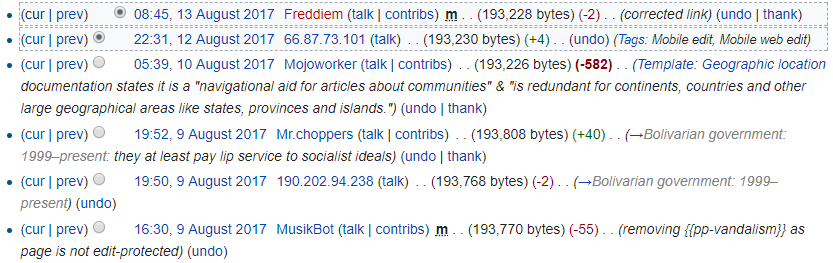
\includegraphics[scale=0.40]{images/marco_teorico/history.png}
    \captionof{figure}{Historial del artículo “Venezuela” en inglés.}
    \label{fig:marco_teorico_history}
    \bigbreak
\end{center}

Cabe destacar que cada versión o cambio provee una serie de propiedades, como: Fecha y hora de la edición, autor de la edición (si el usuario está registrado se refleja su nombre, si no, la dirección ip de su conexión), tamaño del artículo (bytes), bytes modificados, descripción de la edición, selector para identificar si el cambio es menor, y acciones para ejecutar sobre una edición (agradecer o revertir).

\begin{center}
    \bigbreak
    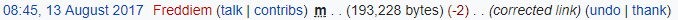
\includegraphics[scale=0.45]{images/marco_teorico/history_detail.png}
    \captionof{figure}{Propiedades de una versión del historial del artículo “Venezuela” en inglés.}
    \label{fig:marco_teorico_history_detail}
    \bigbreak
\end{center}

Adicionalmente, MediaWiki provee un API Web\footnote{\href{https://www.mediawiki.org/wiki/API:Main_page}{Página Principal del API de MediaWiki}}, esto significa que la mayoría de sus funcionalidades están expuesta en la Web y pueden ser accedidas y usadas mediante peticiones HTTP (Hypertext Transfer Protocol). De esta forma, será posible enlazar nuestro trabajo con información de Wikipedia.

\section{Visualización de datos}
La visualización de datos es un medio efectivo y eficiente para comunicar una gran cantidad de información \cite{DesignData}, en donde la comunicación está conformada por elementos visuales, contando con barras, puntos, líneas, colores, figuras, sombras, entre otras. La agrupación de estos elementos visuales se conoce como gráfica.

Como en toda comunicación, es necesario un mensajero, un mensaje y un receptor. En la visualización de datos, el papel del mensajero lo protagoniza un diseñador que codifica la información de manera visual y el receptor es el decodificador del mensaje \cite{DataVis}.

\begin{center}
    \bigbreak
    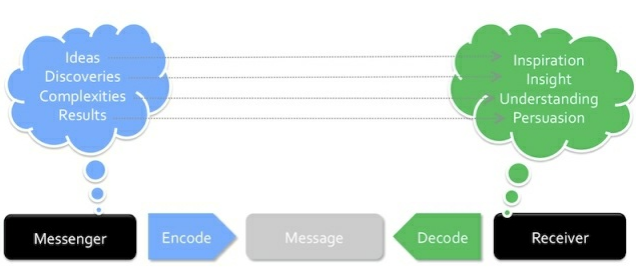
\includegraphics[scale=0.45]{images/marco_teorico/flow_vis.png}
    \captionof{figure}{Diagrama que refleja los actores y acciones de una comunicación visual}
    \label{fig:marco_teorico_flow_vis}
    \bigbreak
\end{center}

El trabajo del mensajero, que en su defecto es el diseñador, desempeña el papel más importante, debido a que tiene que transmitir una información densa usando elementos visuales, por lo tanto tiene que codificar el mensaje lo más claro y simple posible, lo que significa, que tiene que hacer uso correcto de las gráficas y lograr una buena representación de los datos.

\subsection{Enfoque explicativo y exploratorio}
En la visualización de datos se pueden tomar dos enfoques: explicativo y exploratorio.

\textbf{Explicativo:} consta de transmitir una información de manera específica, generalmente, el punto de vista del diseñador de la visualización.

\begin{center}
    \bigbreak
    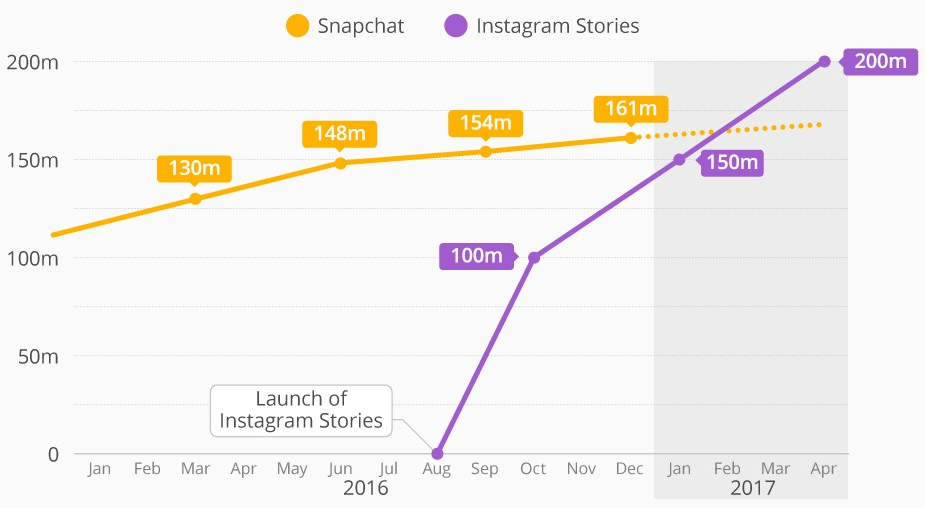
\includegraphics[scale=0.35]{images/marco_teorico/story_chart.png}
    \captionof{figure}{Usuarios activos usando “Historias” de Snapchat vs Instagram}
    \label{fig:marco_teorico_story_chart}
    \bigbreak
\end{center}

En la figura anterior \textbf{Figura \ref{fig:marco_teorico_story_chart}}, se contempla un enfoque explicativo, en donde el diseñador quiere transmitir una información concreta, que es una comparativa en el crecimiento de usuarios activos haciendo uso de la funcionalidad \textit{“Historias"}\footnote{Historias o Stories, es una funcionalidad en donde una persona puede publicar una foto durante un período de tiempo, suele ser de 24 horas.} entre la mensajería de imágenes Snapchat y la red social Instagram.

\textbf{Exploratorio:} es un enfoque en donde la gráfica está adaptada para que el receptor pueda analizar y explorar en ella, y así detectar patrones y relaciones en los datos. Este tipo de gráficas por lo general no suelen transmitir una historia como el enfoque explicativo.

\begin{center}
    \bigbreak
    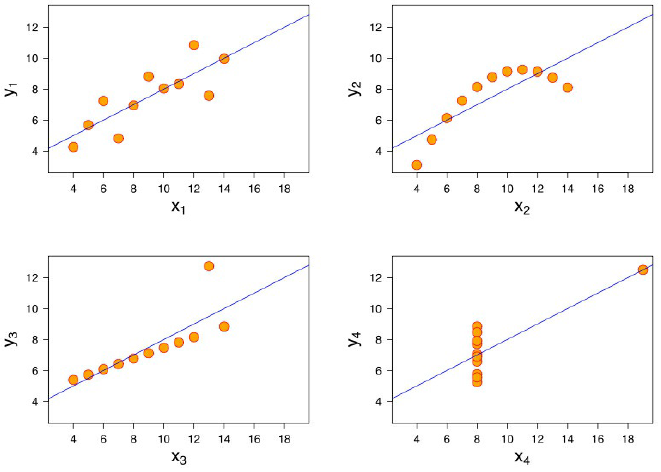
\includegraphics[scale=0.45]{images/marco_teorico/exploratory_chart.png}
    \captionof{figure}{Mediante una gráfica Scatter Plot, podemos analizar patrones y relaciones}
    \label{fig:marco_teorico_exploratory_chart}
    \bigbreak
\end{center}

En la figura anterior \textbf{Figura \ref{fig:marco_teorico_exploratory_chart}}, cada sub-gráfica representa una relación que existe entre dos (2) atributos. No existe una información concreta a transmitir, por lo tanto queda como tarea de la audiencia analizar y explorar relaciones entre atributos. Por ejemplo, el eje Y3 representa precio y eje X3 representa calidad de un producto, entonces según el comportamiento de la gráfica se interpreta que mientras más costoso es un producto mayor es su calidad.

\subsection{Preparación de los datos}
Visualizar datos no es tan sencillo como parece, en su mayoría estos datos tienen que pasar por una limpieza y procesamiento antes de ser visualizados. Si los datos a visualizar son incorrectos o están incompletos, la visualización transmitirá una información errónea. A continuación se presentarán los pasos recomendados [3] para preparar los datos:

\begin{itemize}
    \item\textbf{Adquisición:} lo principal es encontrar la fuente que nos va proveer los datos (Excel, base de datos, etc). Sin los datos es imposible continuar.
    \item\textbf{Examinación:} suelen existir datos incorrectos o incompletos, por lo tanto se debe realizar una verificación de ellos, como eliminar los duplicados, completar con otra fuente los incompletos, acomodar los datos erróneos o en el peor caso removerlos.
    \item\textbf{Estructurar los datos:} dependiendo del tipo de los datos con que contamos la visualización puede variar. Los tipos de datos se pueden dividir en: categórica nominal, categórica ordinal y cuantitativo.
    \begin{itemize}
        \item Categórica nominal: se distinguen por ser un dato que representa un valor textual. Por ejemplo: Un país, un género, etc.
        \item Categórica ordinal: es un dato nominal que puede representar un valor. Por ejemplo: Medallas Olímpicas (Oro, plata, bronce), Calor o Frío, etc.
        \item Cuantitativo: es un dato que representa un valor numérico, en donde algunos son de escala de intervalo y otros de proporción. Por ejemplo: Fechas, temperatura, precio, edad, etc.
    \end{itemize}
    \item\textbf{Limpiar:} eventualmente algunos datos pueden ser atípicos al resto, esto no dice que sean erróneos, pero pueden hacer ruido en la visualización, es buena opción eliminarlos si ese es el caso.
    \item\textbf{Transformar:} para simplificar la visualización y el análisis de la misma es posible que los datos tengan que sufrir una transformación de tipo o pre-calcular ciertas operaciones en los datos. Por ejemplo: promedio de los precios, categorizar edades (Niño: 0-12, Adolescente: 13- 19, Adulto: 20-50, Anciano: +50).
\end{itemize}

\subsection{Métodos de visualización de datos}
Toda visualización está soportada por un método de clasificación, es decir, tiene un motivo y función. A continuación algunos métodos de clasificación \cite{DataVis}:

\begin{itemize}
    \item Comparar categorías o valores
    \item Mostrar cambios en el tiempo
    \item Mostrar conexiones y relaciones
\end{itemize}

\subsection{Tipos de gráficas según método}
En esta sección se presentarán los tipos de gráficas correspondientes al método o función, mencionadas en la sección anterior, que se quiere aplicar:

\begin{itemize}
    \item\textbf{Comparar categorías:} Gráfica de puntos, Gráfica de barras, Gráfica de barras flotantes, histogramas.
    \begin{center}
        \bigbreak
        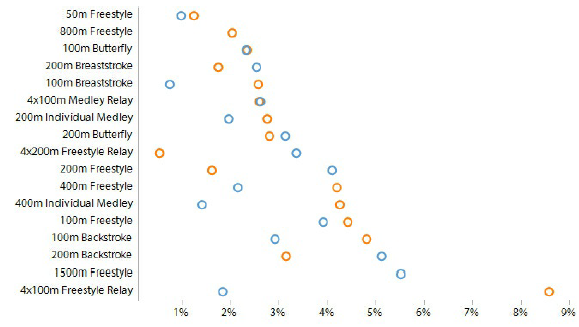
\includegraphics[scale=0.5]{images/marco_teorico/puntos_chart.png}
        \captionof{figure}{Gráfica de puntos}
        \label{fig:marco_teorico_puntos_chart}
        \bigbreak
        
        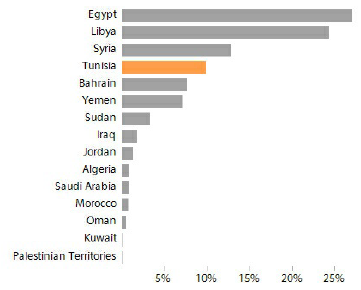
\includegraphics[scale=0.75]{images/marco_teorico/barra_chart.png}
        \captionof{figure}{Gráfica de barras}
        \label{fig:marco_teorico_barra_chart}
        \bigbreak
    
        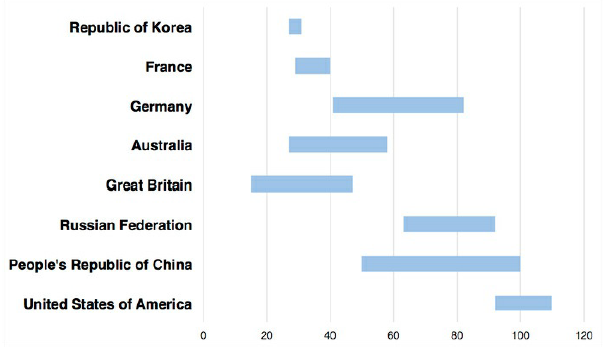
\includegraphics[scale=0.45]{images/marco_teorico/barra_flotante_chart.png}
        \captionof{figure}{Gráfica de barras flotantes}
        \label{fig:marco_teorico_barra_flotante_chart}
        \bigbreak
        
        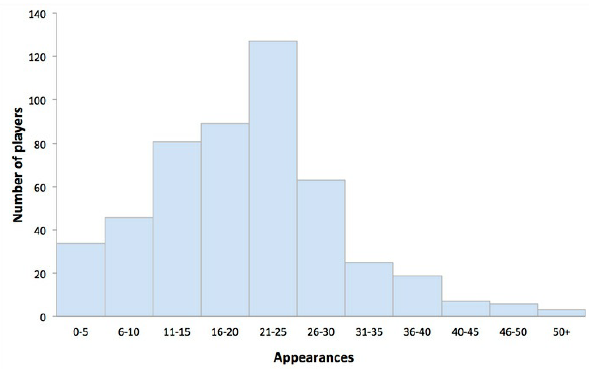
\includegraphics[scale=0.45]{images/marco_teorico/histograma_chart.png}
        \captionof{figure}{Histograma}
        \label{fig:marco_teorico_histograma_chart}
        \bigbreak
    \end{center}
    
    \item\textbf{Cambios en el tiempo:} Gráfica de línea, Gráfica de área, Gráfica de áreas apiladas.
    \begin{center}
        \bigbreak
        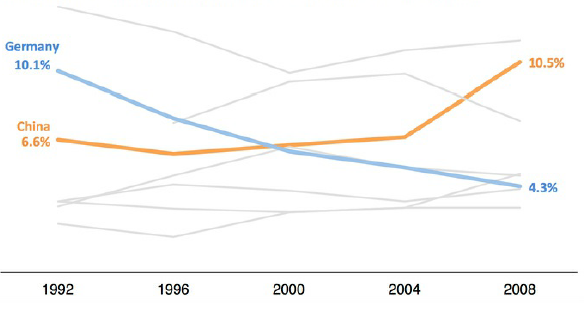
\includegraphics[scale=0.5]{images/marco_teorico/lineal_chart.png}
        \captionof{figure}{Gráfica de lineas}
        \label{fig:marco_teorico_lineal_chart}
        \bigbreak
        
        
        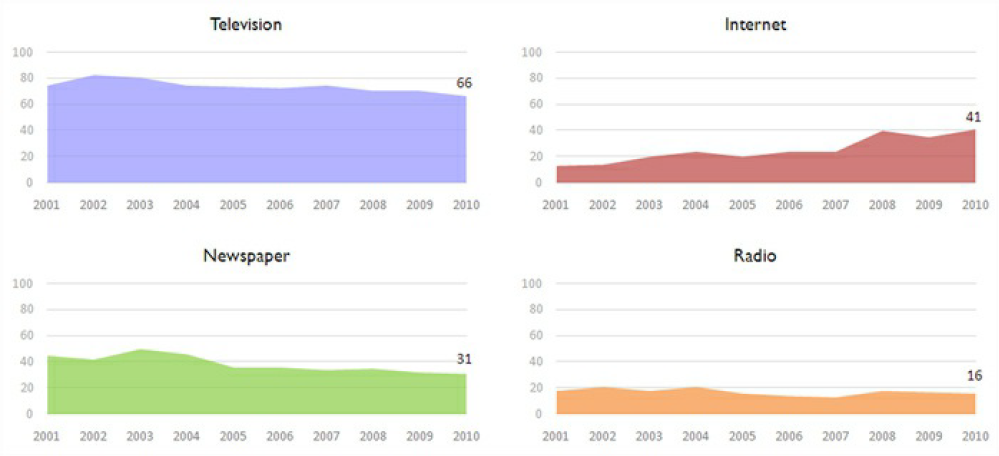
\includegraphics[scale=0.3]{images/marco_teorico/area_chart.png}
        \captionof{figure}{Gráfica de áreas}
        \label{fig:marco_teorico_area_chart}
        \bigbreak
        
        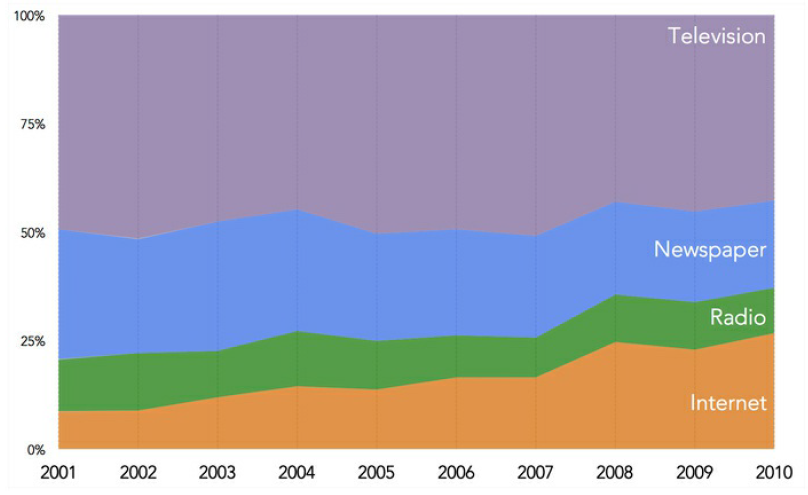
\includegraphics[scale=0.4]{images/marco_teorico/area_apilada_chart.png}
        \captionof{figure}{Gráfica de áreas apiladas}
        \label{fig:marco_teorico_area_apilada_chart}
        \bigbreak
    \end{center}
    \item\textbf{Conexiones y relaciones:} Gráfica de dispersión, Gráfica de burbujas.
    \begin{center}
        \bigbreak
        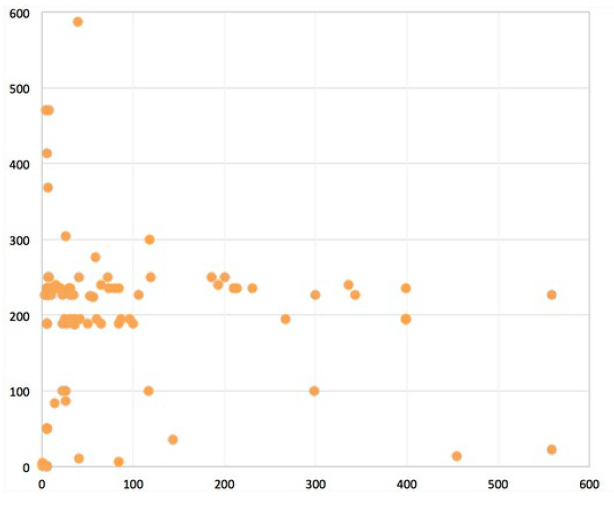
\includegraphics[scale=0.5]{images/marco_teorico/dispersion_chart.png}
        \captionof{figure}{Gráfica de dispersión}
        \label{fig:marco_teorico_dispersion_chart}
        \bigbreak
        
        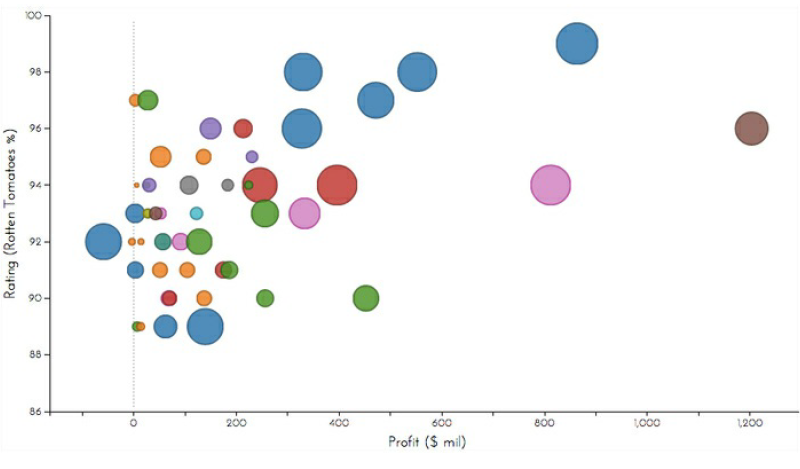
\includegraphics[scale=0.4]{images/marco_teorico/burbuja_chart.png}
        \captionof{figure}{Gráfica de burbujas}
        \label{fig:marco_teorico_burbujas_chart}
        \bigbreak
    \end{center}
\end{itemize}

% Marco Tecnológico
\chapter{Marco Tecnológico}
Este capítulo cubre la investigación y evaluación dada sobre herramientas de apoyo posibles a usar en el trabajo para simplificar el desarrollo. El capítulo inicia introduciendo aquellas herramientas que facilitan las construcción de las visualizaciones sobre los datos. Por último, el capítulo presenta las herramientas que soportan, optimizan y simplifican el desarrollo general de la aplicación web.

\section{Tecnologías para la visualización de datos en web}
Para comenzar, hay que saber que las visualizaciones para este caso se construirán en el ámbito web, haciendo uso de HTML \cite{MozHTML} y JavaScript \cite{MozJS}. De las bibliotecas que nos apoyaremos, algunas construyen la gráfica utilizando el componente Canvas \cite{MozCanvas} de HTML5 y otras utilizando el estándar SVG \cite{W3SVG} (Scalable Vector Graphics).

\subsection[SVG vs Canvas]{SVG vs Canvas \cite{OperaSVGCanvas}}
El elemento Canvas es literalmente, un lienzo donde se va a pintar la gráfica, el proceso de construcción es más complejo y manual ya que la manera para dibujar consiste en pintar pixel por pixel, por lo que el cambio de resoluciones afecta lo dibujado. El elemento SVG (Scalable Vector Graphics) representa un vector escalable, donde cada elemento de la gráfica, ya sea una caja, círculo, texto, o imagen representa un sub-elemento del SVG general. Adicionalmente SVG permite el manejo de eventos y los cambios de resoluciones no afectan la visualización, esto hace que sea más fácil trabajar y personalizar los elementos de la gráfica a dibujar.

Como usaremos bibliotecas para la creación de las gráficas no debemos preocuparnos por la dificultad que toma la construcción con Canvas comparado con SVG, ya que la biblioteca lo hará por nosotros. El punto importante es que Canvas tiene un rendimiento mayor que el SVG cuando la gráfica maneja muchos objetos, debido a que cada objeto de la gráfica es un elemento que impacta en el DOM \cite{W3DOM} del HTML y esto hace que más memoria RAM sea consumida.

\subsection{Bibliotecas basadas en Canvas}
A continuación se presentará una lista de bibliotecas que construyen las gráficas haciendo uso de Canvas, acompañada de una lista de las gráficas principales que incluyen:

\begin{itemize}
\item\textbf{Processing.js\footnote{\url{http://processingjs.org/}}:}
Es un lenguaje de programación visual. Al ser un lenguaje de programación visual queda claro que su objetivo es general y no únicamente gráficas, por lo que nos permite elaborar desde animaciones hasta juegos. Basta con aprender sus definiciones propias para poder usarlo.
\item\textbf{Chartjs\footnote{\url{http://www.chartjs.org/}}:}
Biblioteca con aporte de 5 tipo de gráficas: gráfica de línea, barra, área polar, circular (dona), dispersión. En particular, las gráficas de esta biblioteca presentan un buen diseño adaptativo a distintos tipos de pantalla que pueden ser personalizado, incluyendo animaciones. Adicionalmente, podemos extender las funcionalidades descargando y configurando \textit{plugins} elaborados por otras personas.
\item\textbf{Echarts\footnote{\url{https://ecomfe.github.io/echarts-doc/public/en/index.html}}:}
Posee una gran variedad de gráficas personalizables y dando la posibilidad de habilitar animaciones. Ofrece soporte para la mayoría de los navegadores web y buena usabilidad para los dispositivos móviles, tanto rendimiento como adaptabilidad a la pantalla. La biblioteca con todas las gráficas y componentes incluidos ocupa alrededor de 500KB, pero es posible solo descargar algunos tipos de gráficas para reducir el tamaño de la biblioteca. Entre las gráficas disponibles se tienen: gráfica de línea, barra, área, mapa, circular (dona), dispersión, velas, grafos, boxplot, paralela, embudo y \textit{themeriver} (variación temática sobre el tiempo).
\end{itemize}

\subsection{Bibliotecas basadas en SVG}
A continuación se presentará una lista de bibliotecas que construyen las gráficas haciendo uso de SVG, acompañada de una lista de las gráficas principales que incluyen:

\begin{itemize}
\item\textbf{Raphael.js\footnote{\url{http://dmitrybaranovskiy.github.io/raphael/}}:}
Es una pequeña biblioteca \textit{cross-browser}, es decir, soportada por las mayoría de los navegadores web, con la capacidad de ofrecernos herramientas para elaborar cualquier visualización con vectores. No está orientada solo a la elaboración de gráficas, por lo que podemos crear cualquier visualización, ya sea juegos, alguna especie de arte o animación.
\item\textbf{Google Chart\footnote{\url{https://developers.google.com/chart/}}:}
Biblioteca elaborada por Google, donde ofrecen aproximadamente 29 tipos de gráficas, animadas, con un estilo minimalista y soporte para muchos navegadores, incluyendo versiones viejas. Además, nos permite configurar y personalizar las gráficas a nuestro gusto. La biblioteca solo ocupa 70 KB. Entre los tipos de gráficas disponibles destacan: gráfica de línea, barra, área, mapa, circular (dona), dispersión, intervalos, boxplot, velas, treemap y línea en el tiempo.
\item\textbf{Plotly.js\footnote{\url{https://github.com/plotly/plotly.js/}}:}
Es una biblioteca que está basada (construida) con ayuda de la biblioteca D3 y stackgl\footnote{Es un ecosistema para WebGL \url{http://stack.gl/}}. Tiene 20 tipos de gráficas, incluyendo en 3D (tres dimensiones) con un diseño agradable y con una cómoda caja de herramientas flotante para interactuar con la gráfica. Entre los tipos gráficas disponibles se tienen: gráfica de línea, barra, área, circular (dona), mapa, dispersión, boxplot, velas, treemap e histogramas (2D y 3D).
\end{itemize}


\subsection{D3 (Data-Driven Documents)}
D3 (Data-Driven Documents)\footnote{\url{https://d3js.org/}} es considerada una de las bibliotecas más potentes para la manipulación de datos, con varios años en desarrollo y con una comunidad bastante activa. Con esta biblioteca se puede llegar a construir casi cualquier tipo de gráfica deseable en SVG o HTML Canvas, gracias a que tenemos un control total sobre la construcción y diseño de la gráfica. También se dispone de \textit{plugins} y gran cantidad de ejemplos aportados por otras personas que pueden ayudarnos a facilitar la programación de la gráfica. La biblioteca tiene un tamaño base de 230 KB aproximadamente en su versión actual (v4.7.3).
Para hacer posible la construcción de una gráfica, D3 incluye los siguientes elementos claves:

\begin{itemize}
\item\textbf{Selecciones}: modificar elementos de manera imperativa, siendo menos tediosa a la tradicional
\begin{minted}[linenos]{js}
    d3.selectAll('p').style('color', 'white');
\end{minted}
Podemos modificar atributos o estilos, registrar eventos, agregar, eliminar nodos logrando cambiar HTML o texto contenido.

\item\textbf{Propiedades dinámicas}: los estilos, atributos y otras propiedades pueden ser especificadas como funciones de datos, es decir no siempre reciben constantes.
\begin{minted}[linenos]{js}
d3.selectAll("p").style("color", function() {
  return "hsl(" + Math.random() * 360 + ", 100%, 50%)";
});
\end{minted}

\item\textbf{Entrar y salir}: facilita agregar y/o remover elementos en un grupo de datos.
\begin{minted}[linenos]{js}
var p = d3.select("body")
  .selectAll("p")
  .data([4, 8, 15, 16, 23, 42])
    .text(function(d) { return d; });

// Entrar
p.enter().append("p")
    .text(function(d) { return d; });

// Salir
p.exit().remove();
\end{minted}
En casos donde se busca optimizar esta sección es útil debido a que podemos establecer una navegación en la visualización y solo mostrar un grupo de elementos donde el resto se elimina, de tal forma que se vayan agregando y eliminando elementos a medida que se realicen acciones sobre la gráfica. 

\item\textbf{Transiciones}: existen controles para las animaciones, como la duración y tiempo de aplazo.
\begin{minted}[linenos]{js}
d3.selectAll("circle").transition()
    .duration(750)
    .delay(function(d, i) { return i * 10; })
    .attr("r", function(d) { return Math.sqrt(d * scale); });
\end{minted}
\end{itemize}
La biblioteca D3 no introduce una nueva representación visual como hace Raphael.js y Processing.js (bibliotecas mencionadas anteriormente), debido a que se trabaja directamente con estándares web (HTML, CSS \cite{MozCSS}, SVG), por ejemplo, podemos crear una gráfica en SVG y luego darle estilo con un archivo externo CSS. Sin embargo, estas tres (3) bibliotecas por el hecho de darnos una libertad total al construir visualizaciones requieren un tiempo considerado para aprender y poder usarlas debidamente.

\subsection{Evaluación de Bibliotecas}
Es importante saber que para nuestro caso todas las bibliotecas mencionadas anteriormente son las que mejor se adaptan según las necesidades, aún así se realizaron ciertas evaluaciones para decidir cuál utilizar. Para la evaluación se consideró lo siguiente:

\begin{itemize}
\item \textbf{Variedad de gráficas}

Para nuestro trabajo es necesario varios tipos de gráficas, ya que se realizarán visualizaciones con cantidad y tipo de datos distintos, por lo tanto es indispensable que existan diferentes tipos de gráficas para cada situación a visualizar en particular. Se revisó todos los tipos de gráficas que podían ofrecer cada una de las bibliotecas. Si es necesario un diseño o tipo de gráfica bastante particular probablemente para ese caso la mejor opción sería D3, Raphael.js o Processing.js.

\item \textbf{Rendimiento}

Definimos rendimiento como el comportamiento que toma la biblioteca al construir una gráfica considerablemente pesada (con inmensa cantidad de datos). El problema que podemos presentar al visualizar grandes cantidades de datos es que la vista donde está la gráfica se perciba con cierta lentitud y en el peor de los casos el navegador (browser) se detenga, es decir deje de trabajar. Afortunadamente, hay algunas bibliotecas que optimizan las gráfica y aplican un estilo de paginación, donde no dibujan todos los puntos a la vez, sino a medida que nos profundizamos en la gráfica.

Se sometieron algunas de las bibliotecas a la creación de una gráfica desde 10.000 hasta 1.000.000 de datos. En la \textbf{Figura \ref{fig:library_comparison}} podemos apreciar una aproximación del resultado basado en la cantidad de objetos que pudieron soportar, en donde el eje 'y' corresponde al número de objetos, donde M representa el millón. Cabe destacar que D3, Processing y Raphael no fueron considerados ya que su rendimiento es totalmente relativo a como se programe la gráfica.
\begin{center}
    \bigbreak
    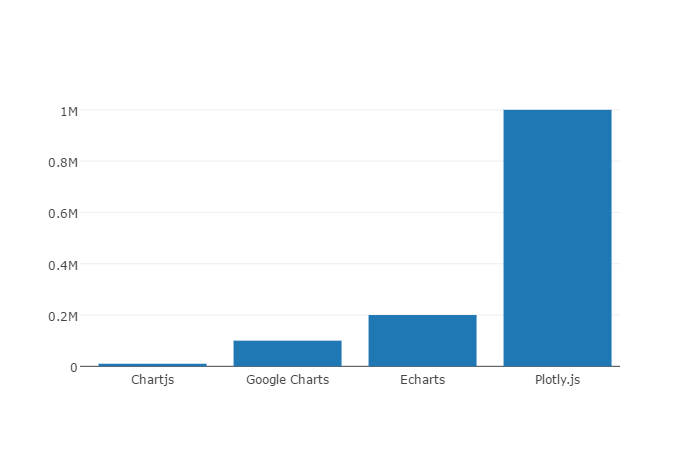
\includegraphics[scale=0.45]{images/marco_tecnologico/library_comparison.png}
    \captionof{figure}{Comparación de bibliotecas de visualización}
    \label{fig:library_comparison}
    \end{center}
    \bigbreak
\end{itemize}

Al analizar la evaluación, quedamos con tres (3) candidatos: D3, Echarts y Plotly. Donde cada uno predomina en distintos escenarios necesarios para nuestro trabajo. Adicionalmente, D3 al ser una biblioteca que nos ofrece la mayor libertad para elaborar gráficas a nuestro gusto dará aquel soporte en gráficas sumamente específicas, también viene acompañada de muchos ejemplos elaborados por la comunidad que pueden servir de apoyo. Plotly a pesar de construir las visualizaciones en SVG logra un excelente rendimiento, aún mejor que el resto de las bibliotecas, además su diseño es agradable y nos ofrece una caja de herramientas para interactuar con la gráfica. Como último candidato a Echarts, por su gran variedad de ejemplos y los posibles tipos de gráficas que nos puede ofrecer, agregando que, dan soporte con gráficas que son usables en dispositivos móviles logrando además un buen rendimiento para aquellos sistemas de bajos recursos.

\section{Tecnologías para el desarrollo web}
Brindar una buena experiencia de usuario en una aplicación puede llegar a ser un gran desafío donde existen varios elementos que afectan directamente, como el \textbf{diseño}, ya que es importante jugar un buen estilo, de carácter agradable, y con animaciones amigables. El \textbf{rendimiento}, donde la aplicación debe desempeñar una buena fluidez de respuesta y \textbf{correctitud}, que se contemple una interfaz que tenga sentido con la funcionalidad de la misma.

Cuando entramos en el área web, nuestro caso una aplicación web, llegan algunos desafíos adicionales como aplicar soporte de diseño para variedad de densidades de pantallas y versiones de navegadores web, esto se debe a que nuestra aplicación estará expuesta en la web, donde puede ser accedida desde tabletas, móviles, computadores de escritorio, televisores, y cualquier dispositivo que tenga conexión a internet y un navegador. También el peso de la aplicación, incluyendo códigos, fuentes e imágenes impacta considerablemente al tiempo de espera para conexiones lentas a internet.

En este capítulo presentaremos herramientas que nos facilitarán el trabajo para lidiar las problemáticas mencionadas segmentando la aplicación por: arquitectura, diseño y utilidades extras a emplear. Cabe acotar que para el manejo de estas herramientas es necesario tener conocimiento sobre JavaScript, TypeScript\footnote{TypeScript \url{https://www.typescriptlang.org/}} (subconjunto de JavaScript con un sistema de tipos más robusto), CSS y HTML.

\subsection{Arquitectura}

La aplicación adoptará una arquitectura llamada \textit{Single-page Aplication} \cite{WikiSPA} (SPA) que significa aplicación de una página, donde se busca englobar toda la aplicación en una vista, logrando cargar la base de la aplicación completa y luego dinámicamente mediante JavaScript hacer la transición de las vistas. La gran ventaja que podemos sacar de SPA es la fluidez de la aplicación entre cambios de vistas, ya que todos estos elementos ya fueron cargados previamente. Por contraparte, la carga inicial suele ser pesada por traerse elementos de más, pero de igual forma esta puede optimizarse para traer solo los recursos necesarios.

Mayormente nuestra aplicación tendrá comunicación casi constante con un API que nos ofrecerá cantidades de datos para nosotros transmitir visualmente, por lo tanto manejaremos peticiones HTTP\footnote{HTTP: es el protocolo de comunicación que permite las transferencias de información en la World Wide Web.} (Hypertext Transfer Protocol) con AJAX \cite{AJAX} (Asynchronous JavaScript And XML), cabe destacar que al ser asíncrono evitamos que afecte el flujo principal de la aplicación.
\begin{center}
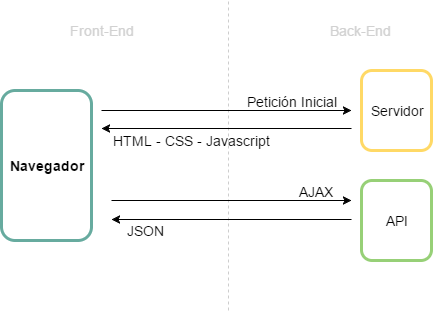
\includegraphics[scale=0.6]{images/marco_tecnologico/spa_lifecycle.png}
\captionof{figure}{Ciclo de vida de una aplicación SPA}
\label{fig:spa_lifecycle}
\end{center}
El ciclo de una aplicación SPA como se muestra en la \textbf{Figura \ref{fig:spa_lifecycle}} requiere por lo general una primera petición para cargar las vistas, funciones y diseño, el resto de las peticiones se dirigen al API a través de AJAX para pedir los datos a visualizar.

A continuación presentaremos dos (2) bibliotecas que nos permiten definir la aquitectura de la aplicación: Angular y jQuery.

\subsubsection{Angular}
Angular\footnote{Angular 2 \url{https://angular.io/}} es un framework muy popular creado por Google destinado a construir aplicaciones web, donde se maneja la lógica de la aplicación con JavaScript. Para la versión 2 de Angular, que es la que se contempla para este proyecto, se logra una estructura modular en la aplicación, donde cada elemento es considerado un componente que se construye de manera aislada, por lo tanto no se ve afectado por el resto de los mismos. Claramente, el enfoque de Angular sigue la arquitectura SPA, donde logra optimizar y resolver posibles problemas con los estados de transiciones, carga inicial, caching y mejor manejo de peticiones HTTP.

Es importante saber que Angular es una biblioteca con un catálogo inmenso de funcionalidades soportado por la mayoría de los navegadores, donde ofrece desde mecanismos de seguridad para evitar \textit{Cross-site scripting}\footnote{Cross-site scripting \url{https://es.wikipedia.org/wiki/Cross-site_scripting}} (XSS) hasta un paquete completo de animaciones.

A continuación, se muestra un ejemplo de código representando un componente en Angular:
\begin{minted}[linenos]{ts}

// app.component
import { Component } from '@angular/core';

@Component({
  selector: 'my-app',
  template: `<h1>Hola Mundo</h1>`
})
export class AppComponent { name = 'Angular'; }
\end{minted}

Podemos observar que para declarar un componente es necesario importar primero el paquete de Angular y luego llamar al decorador \textbf{@Component({})}, en donde es pasado un objeto identificado por un \textbf{selector}, que corresponde a un alias del componente y el \textbf{template} que puede ser una ruta de un archivo HTML o este caso una pieza de código HTML.

\begin{minted}[linenos]{ts}
// app.module
import { NgModule }      from '@angular/core';
import { BrowserModule } from '@angular/platform-browser';
import { AppComponent }  from './app.component';

@NgModule({
  imports:      [ BrowserModule ],
  declarations: [ AppComponent ],
  bootstrap:    [ AppComponent ]
})
export class AppModule { }
\end{minted}

Es indispensable al menos un módulo en Angular por lo tanto en el código anterior estamos definiendo un módulo con el decorador \textbf{@NgModule({})}, lo importante de aquí es que en dicho módulo declaramos el componente anteriormente creado.

Otras características que destacan a Angular son:

\begin{itemize}
\item\textbf{Directivas}

Es una manera de lograr que las vistas sean dinámicas, es decir, los componentes HTML pueden tener atributos especiales de Angular para poder modificar elementos del DOM.
\begin{minted}[linenos]{html}
<li *ngFor="let item of arrayItem"></li>
<app-detail *ngIf="selectedItem"></app-detail>
\end{minted}
La directiva \textbf{*ngFor} nos permite iterar en un ciclo, originando un <li> por cada elemento de arrayItem y \textbf{*ngIf} nos permite mostrar o no elementos mediante una condición.

\item\textbf{Servicios}

Pueden representar cualquier función, valor o características que la aplicación necesite. Mayormente los componentes son consumidores de estos servicios, por ejemplo: una configuración de la aplicación, un servicio que hace peticiones HTTP a un API, un servicio encargado de actualizar una barra de navegación, un servicio para mostrar mensajes estilo Logs, etc.
\begin{minted}[linenos]{ts}
// logger.service.ts
export class Logger {
  log(msg: any)   { console.log(msg); }
  error(msg: any) { console.error(msg); }
  warn(msg: any)  { console.warn(msg); }
}
\end{minted}
El código de arriba representa un ejemplo de un servicio de Logs, en donde nos ofrece una clase con tres (3) variedades de avisos a consola.
\end{itemize}

\subsubsection{jQuery}
jQuery\footnote{jQuery \url{https://jquery.com/}} es una biblioteca ligera y sencilla, que lleva bastante tiempo siendo usada. Su finalidad es ofrecer soluciones a funciones complejas de manera sencilla principalmente para la manipulación de elementos HTML y eventos, animaciones y AJAX. Considero jQuery como una opción manual al construir una aplicación SPA, ya que directamente no ofrece una solución completa, pero existen plugins y/o guías para lograr dicha arquitectura.

\begin{itemize}

\item\textbf{Manipulación de elementos}
\begin{minted}[linenos]{js}

$( "button.green" ).html( "Next" );

\end{minted}

\item\textbf{Manejo de Eventos}
\begin{minted}[linenos]{js}
var hiddenBox = $( "#banner-message" );
$( "#button-container button" ).on( "click", function( event ) {
  hiddenBox.show();
});
\end{minted}

\item\textbf{Petición HTTP Asíncrona con AJAX}
\begin{minted}[linenos]{js}
$.ajax({
  url: "/api/getWeather",
  data: {
    zipcode: 97201
  },
  success: function( result ) {
    $( "#weather-temp" )
    .html( "<strong>" + result + "</strong> degrees" );
  }
});
\end{minted}
\end{itemize}

\subsection{Diseño}

Es importante que nuestra aplicación presente un buen diseño, donde se simplifique la finalidad de la aplicación, además de ser capaz a adaptarse a distintos tamaños de pantallas. No hay un guion o estilo definido para el diseño, la idea es aplicar colores que combinen, componentes sencillos como: botones, selectores, barra de menú, diálogos, iconos, \textit{inputs} (entradas de información), texto y componentes no tan sencillos como las gráficas para visualizar los datos. Todos estos componentes harán posible una interfaz que sea capaz de representar un editor de visualizaciones, en donde recibiremos apoyo de bibliotecas que nos ofrecen estos componentes bien formados y listos para usar.

\subsubsection{Angular Material}

Angular Material\footnote{Angular Material \url{https://material.angular.io/}} es una biblioteca que ofrece componentes siguiendo un diseño llamado Material (Material Design)\footnote{Material Design \url{https://material.io/}} creado por Google. Para poder integrar esta biblioteca es requerido Angular 2, por lo tanto, esta opción se ve atada a usar dicho framework. Lo que destaca de Angular Material es la variedad de componentes, que además son totalmente adaptativos gracias a una biblioteca incluida llamada \textit{Flex Layout}\footnote{Flex Layout \url{https://github.com/angular/flex-layout}} que nos ofrece propiedades sencillas de usar para corresponder el tamaño de los componentes en distintos escenarios. Adicionalmente, es soportado por la mayoría de los navegadores modernos.

Angular Material al estar atado al framework nos da la posibilidad de exportar sólo los componentes que necesitemos y no todos los de la biblioteca, además nos permite añadir soporte de gestos a los componentes como \textit{toggle} o \textit{slider}.

Entre tantos componentes, se mostrará ejemplos de algunos a continuación:

\begin{itemize}
\item\textbf{Botones}
\begin{minted}[linenos]{html}
<button md-raised-button>Raised button</button>
<button md-fab><md-icon>check</md-icon></button>
\end{minted}
En donde el atributo \textbf{md-raised-button} representa un botón con elevación, \textbf{md-fab} es un botón mayormente flotante con forma circular. Podemos observar que existe otro elemento \textbf{md-icon} que nos permite colocar un ícono a través de una fuente especial llamada \textit{Material Design Icons}\footnote{Material Design Icons \url{https://material.io/icons/}}, obteniéndola con el siguiente código desde nuestro archivo HTML.
\begin{minted}[linenos]{html}
<link
href="https://fonts.googleapis.com/icon?family=Material+Icons"
rel="stylesheet">
\end{minted}

\item\textbf{Spinner de Progreso}
\begin{minted}[linenos]{console}
<md-progress-spinner
    class="example-margin"
    [attr.color]="color"
    [mode]="mode"
    [value]="value">
</md-progress-spinner>
\end{minted}
El \textit{spinner}, que hace referencia a un elemento circular con acción de progreso, se puede lograr usando \textbf{md-progress-spinner} en donde puede tener como atributo un color, un modo para representar si girará finitamente o infinitamente y un valor que representa el porcentaje de progreso actual.

\item\textbf{Barra de Herramientas}
\begin{minted}[linenos]{html}
<md-toolbar>My App</md-toolbar>
\end{minted}
Con \textbf{md-toolbar} logramos crear una barra en donde podremos colocar texto e iconos con acciones, por ejemplo, la barra principal superior de la aplicación.
\end{itemize}


\subsubsection{Bootstrap}

Bootstrap\footnote{Bootstrap \url{http://getbootstrap.com/}} ofrece un gran catálogo de componentes, desde distintos tipos de botones, formularios, barras de menú, hasta diálogos. Recientemente lanzaron la versión 4, en donde se reescribió la mayoría del proyecto corrigiendo bastantes errores, sin embargo esta versión se encuentra en fase alfa, esto quiere decir que no es estable. Bootstrap es una biblioteca elaborada por Twitter, donde es posible la construcción rápida de una interfaz tanto para escritorio como para móvil, ofreciendo gran soporte para la mayoría de los navegadores y también posibilidad de adaptarse a distintas dimensiones de pantallas. Para que Bootstrap funcione es necesario la biblioteca jQuery que anteriormente mencionamos.

Bootstrap tienen su propio sistema \textit{grid} para escalar los componentes según cambie el tamaño de la pantalla, en donde se distinguen tres medidas: \textbf{lg} (largo), \textbf{md} (mediano), \textbf{sm} (pequeño) y \textbf{xs} (extra pequeño). Estas medidas pueden aplicarse a columnas o filas, representadas como \textbf{col} y \textbf{row}. Por cada fila puede haber doce (12) columnas, si este es superado el elemento faltante irá posicionado abajo.
\begin{minted}[linenos]{html}
<div class="row">
  <div class="col-md-4">.col-md-4</div>
  <div class="col-md-4">.col-md-4</div>
  <div class="col-md-4">.col-md-4</div>
</div>
<div class="row">
  <div class="col-xs-12 col-md-8">.col-xs-12 .col-md-8</div>
  <div class="col-xs-6 col-md-4">.col-xs-6 .col-md-4</div>
</div>
\end{minted}

Entre los componentes considerados a usar:
\begin{itemize}
\item\textbf{Botones}
\begin{minted}[linenos]{html}
<button type="button" class="btn btn-default">Default</button>
<button type="button" class="btn btn-primary">Primary</button>
<button type="button" class="btn btn-success">Success</button>
<button type="button" class="btn btn-info">Info</button>
<button type="button" class="btn btn-warning">Warning</button>
<button type="button" class="btn btn-danger">Danger</button>
\end{minted}
Bootstrap nos proporciona un abanico de botones con estilos definidos, en donde cada uno juega un color de fondo distinto.

\item\textbf{Tipografía}
\begin{minted}[linenos]{html}
<span class="glyphicon glyphicon-star"
aria-hidden="true"></span> Star
\end{minted}
Es posible incluir íconos gracias a que Bootstrap trae su propia tipografía.

\item\textbf{Barra de Progreso}
\begin{minted}[linenos]{html}
<div class="progress">
  <div class="progress-bar" role="progressbar"
  aria-valuenow="60" aria-valuemin="0"
  aria-valuemax="100" style="width: 60%;">
    <span class="sr-only">60% Complete</span>
  </div>
</div>
\end{minted}

\item\textbf{Barra de Herramientas}
\begin{minted}[linenos]{html}
<nav class="navbar navbar-default">
  <div class="container-fluid">
    <div class="navbar-header">
      <a class="navbar-brand" href="#">
        <img alt="Brand" src="...">
        <h1>Title</h1>
      </a>
    </div>
  </div>
</nav>
\end{minted}
Es posible posicionar una barra superior de manera fija, con cualquier elemento adentro de ella, pero para ellos debes cumplir con los 3 primeros elementos padres: el primer \textbf{nav} y los dos siguientes \textbf{div}.

\end{itemize}


\subsection{Utilidades}

Existen distintas bibliotecas de propósito más específico cuyo uso se ha vuelto cotidiano, donde pueden solucionar tareas complejas o engorrosas de implementar en JavaScript, específicamente para nuestro proyecto existe la necesidad de preparar ciertos conjuntos de datos complejos para poder construir una gráfica, al igual que manejar varios formatos de fechas.

\subsubsection[Lodash]{Lodash\footnote{Lodash \url{https://lodash.com/}}}

La manipulación de ciertos objetos, arreglos y strings complejos pueden contemplar soluciones un tanto ilegible, por lo tanto la biblioteca Lodash nos otorga utilidades que resuelven dichos problemas de una manera simple. Adicionalmente, cuenta con funciones matemáticas y soluciones para manejar valores null, NaN y undefined. Todas sus funcionalidades son soportadas por la mayoría de los exploradores.

A continuación, se mostrarán unos ejemplos de las ventajas que puede traer lodash a nivel de implementación:

\begin{itemize}
\item\textbf{Verificar variable (no sea null ni undefined)}
\begin{minted}[linenos]{js}
// no-lodash
if(a != null && a != undefined) {...}

// lodash
if(!_.isNill(a)) {...}
\end{minted}

\item\textbf{Ciclos}
\begin{minted}[linenos]{js}
// no-lodash
for(var i = 0; i < 5; i++) {
  ...
}

// lodash
_.times(5, function(){
  ...
});
\end{minted}

\item\textbf{Números aleatorios}
\begin{minted}[linenos]{js}
// no-lodash
Math.floor(Math.random() * (max - min + 1)) + min;

// lodash
_.random(min, max);
});
\end{minted}

\item\textbf{Seleccionar elementos de un arreglo}
\begin{minted}[linenos]{js}
// no-lodash
function pick(arr) {
    var _this = this;
    var obj = {};
    arr.forEach(function(key){
        obj[key] = _this[key];
    });

    return obj;
};
objA.pick(['x', 'y'])

// lodash
_.pick(objA, ['x', 'y']);
});
\end{minted}
\end{itemize}

\subsubsection[Moment]{Moment\footnote{Momentjs \url{https://momentjs.com/}}}

La manipulación de fecha y tiempo en JavaScript suele ser confusa y consume muchas líneas de código, es probable que en nuestra aplicación tengamos que recibir fechas con un formato específico y de la misma forma representar este visualmente de otra. Moment es una biblioteca que tiene como finalidad analizar sintácticamente, validar, manipular y mostrar fechas/horas (tiempo) de la forma más simple posible. Adicionalmente, esta biblioteca ofrece extensiones para poder realizar ciertas funcionalidades más específicas.

A continuación mostraremos ejemplos de cosas interesantes que podemos lograr con dicha biblioteca:

\begin{itemize}
\item\textbf{Obtener la fecha/hora de hoy con formato}
\begin{minted}[linenos]{js}
// date
moment().format("DD/MM/YYYY");
// time
moment().format("HH:mm:ss");
\end{minted}

\item\textbf{Agregar/Quitar tiempo}
\begin{minted}[linenos]{js}
// add
moment().add(7, 'days');
moment().add(1, 'week')
// subtract
moment().subtract(7, 'days');
moment().subtract(1, 'week')
\end{minted}

\item\textbf{Obtener unidad de tiempo específica}
\begin{minted}[linenos]{js}
// hours
moment().hours();
// month
moment().month();
\end{minted}
\end{itemize}

\bigbreak
Presentadas estas alternativas, tomaremos Angular para la arquitectura y Angular Material para el diseño respectivamente. Esta selección se justifica debido a que Angular como framework para el front-end tiene un enfoque total SPA, además tiene ciertas herramientas integradas, como un manejador de conexiones http que es de bastante utilidad para nuestro caso. También, Angular orienta a programar de manera modular, en donde se logra un código más organizado y reutilizable. Por el lado del diseño, Angular Material es una buena opción, debido a su compatibilidad con el framework, adicionalmente, posee una gran cantidad de vistas adaptativas totalmente controlables mediante directivas de Angular.

% Marco Aplicativo
\chapter{Marco Aplicativo}
Este capítulo describe la metodología y la ejecución de la misma, explicando cada una de las tareas en orden cronológico de manera detallada y su resultado.

\section{Metodología}
Los objetivos específicos serán desglosados de manera técnica en pequeñas tareas ordenadas por prioridad. El control de estas asignaciones se manejará mediante la plataforma GitHub (aplicación web para alojar repositorios Git) en donde cada tarea será un \textit{issue} a resolver. Github nos permite proyectar estos \textit{issues} en una pizarra, con el fin de visualizar el estado de cada asignación, los estados definidos son: Por hacer, En progreso, Terminado. Puede verse un ejemplo en la \textbf{Figura \ref{fig:githubBoard}}

\begin{itemize}
\item\textbf{Por hacer:} representa aquellas tareas especificadas, que por el momentos son \textit{issues} sin resolver.
\item\textbf{En progreso:} representa las tareas que están siendo desarrolladas, cabe destacar que cada asignación se resuelve en una rama distinta del repositorio git haciendo uso del \textit{pull request} para llevar un mayor control del desarrollo de la asignación.
\item\textbf{Terminado:} representa aquellas tareas culminadas. Cuando se considera que una tarea está lista, esta tiene que ser mezclada a la rama principal del repositorio, llamada \textit{master}, luego cerrar el \textit{pull request} y el \textit{issue} asociado.
\end{itemize}

\begin{center}
    \bigbreak
    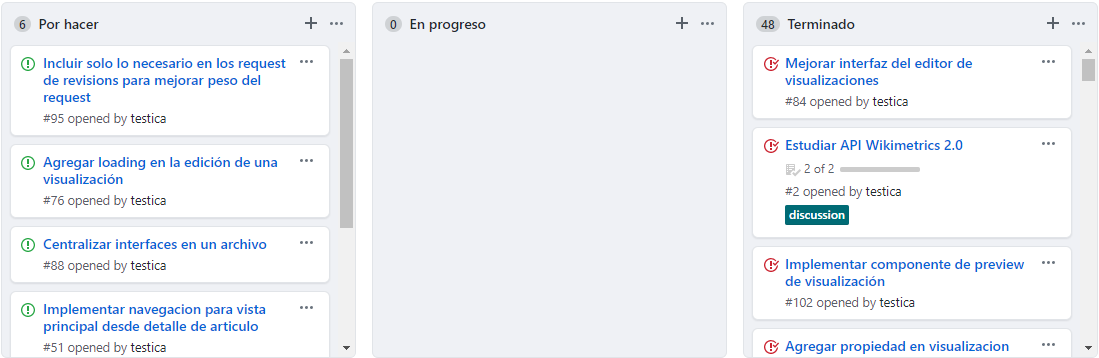
\includegraphics[scale=0.4]{images/marco_aplicativo/github_board.png}
    \captionof{figure}{Pizarra de Github}
    \label{fig:githubBoard}
    \bigbreak
\end{center}

La pizarra de Github es una herramienta de la metodología Kanban \cite{BookKanban}, en donde visualizar el flujo de trabajo y hacerlo visible es la base para comprender cómo avanza el trabajo. Sin comprender el flujo de trabajo, realizar los cambios adecuados es más difícil. Una forma común de visualizar el flujo de trabajo es el uso de columnas. Las columnas representan los diferentes estados o pasos en el flujo de trabajo. Kanban logra un desarrollo evolutivo e incremental, donde las soluciones de las asignaciones puede que no sean las mejores comenzando, pero a medida que se itera se va perfeccionando.

\section{Realización de tareas}
A continuación, de listarán las tareas de mayor relevancia ordenadas cronológicamente, con la descripción del problema y el resultado.

\begin{enumerate}
  \item\textbf{Preparar entorno de desarrollo:}\\
  
  Antes de empezar el desarrollo es necesario instalar o preparar el ambiente para el uso de las herramientas:
  \begin{itemize}
      \item Instalar Node\footnote{\url{https://nodejs.org}} para servir la aplicación web local.
      \item Instalar NPM\footnote{\url{https://www.npmjs.com/}} (Node Package Manager) necesaria para instalar paquetes javascript como Angular y dependencias.
      \item Instalar editor de texto inteligente, en preferencia personal, Visual Studio Code.
      \item Instalar algún navegador moderno, Google Chrome o Firefox para reproducir la aplicación web.
  \end{itemize}
  
  \item\textbf{Elaborar estructura base de la aplicación:}\\
  Lo principal es tener la estructura base del proyecto en código, tener la configuración del framework Angular lista.
  
  Afortunadamente, existe una herramienta llamada \textbf{angular-cli}, que nos facilita la creación de un proyecto en Angular poniendo lo siguiente en el terminal:
  \begin{minted}[linenos]{console}
    # instalar angular-cli
    npm install -g @angular/cli
    # crear proyecto
    ng new wiki-history-client
  \end{minted}
  
  \item\textbf{Investigar API de WikiMedia:}\\
  
  Necesitamos ofrecer los artículos del watchlist de los usuarios para que posteriormente puedan analizarlos con la aplicación, dado esto es necesario saber como autenticar un usuario y obtener su watchlist haciendo uso del API.
  
  En el momento cuando se desempeñó esta tarea hubo un problema con el API de autenticación, debido a que estaban abandonando la manera tradicional y migrando a una más segura usando OAuth2\footnote{\url{https://oauth.net/2/}}, por temas de burocracia no fue posible registrar nuestra aplicación con su método nuevo de autenticación.
  
  Debido a esto, no iba a ser posible extraer el watchlist sin credenciales de usuarios, por lo que se optó la decisión de construir un API propia donde se gestionaran usuarios y ellos manualmente agregarían los artículos de interés.
  
  \item\textbf{Implementar vista de Artículos:}\\
  
  La vista principal de la aplicación sería una lista de artículos de interés.
  
  Por el momento, los datos de los artículos se simularon en una variable, para probar que la vista funcionaba.
  \begin{center}
      \bigbreak
      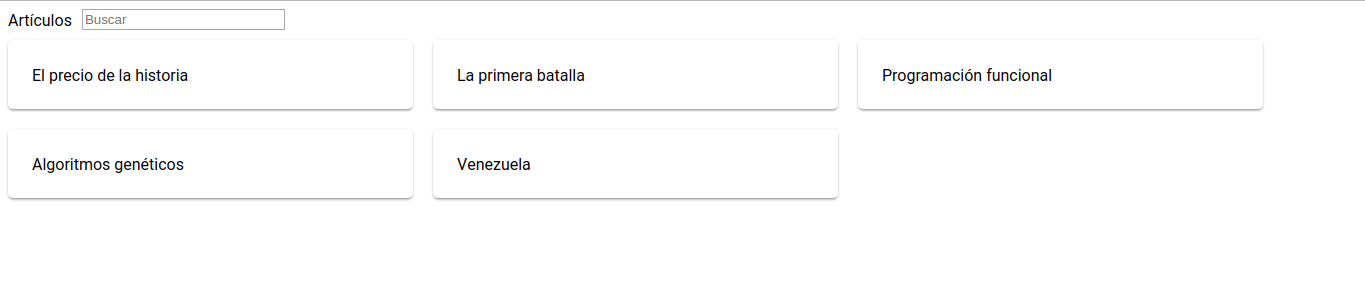
\includegraphics[scale=0.2]{images/marco_aplicativo/lista_articulos.png}
      \captionof{figure}{Lista de artículos}
      \label{fig:githubBoard}
      \bigbreak
  \end{center}
  
  Usamos un elemento de Angular Material llamado md-card, para formar el estilo de un artículo. La propiedad *ngFor es una directiva de angular que nos permite replicar ese elemento tanta veces como iteraciones tenga. Además hacemos uso de fxFlex que nos permite ajustar el tamaño del elemento dependiendo de las dimensiones de la pantalla.
  \begin{minted}[linenos]{html}
    <md-card 
        *ngFor="let article of articles"
        fxFlex="30" fxFlex.sm="50" fxFlex.xs="100">
        {{article.title}}
    </md-card>
  \end{minted}
  
  \item\textbf{Implementar vista de detalle de  Artículo:}\\
  Al presionar un artículo de la lista nos tiene que  dirigir a un detalle para acceder a más información del mismo.
  
  Por el momento simplemente mostraremos una vista blanca que representa el detalle. De esta forma, programamos que al pisar un artículo nos mande a la vista del detalle. La ruta del detalle se representa por: 
  \begin{minted}{console}
   /articles/<titulo_artículo>
  \end{minted}
  
  \item\textbf{Implementar servicio (API) para manejar usuarios y configuraciones:}\\
  
  Es necesario un servicio que delegue la autenticación y gestión de los recursos persistentes como usuarios y artículos.
  
  Se desarrolló un API usando el micro framework Python Flask\footnote{\url{flask.pocoo.org/}} y para la persistencia de los datos se usó MongoDB, se consideró una base de datos NoSQL debido a que los datos no están relacionados, son simplemente usuarios con configuraciones personales.
  
  Se implementaron las siguientes rutas en el API:
  \begin{minted}{console}
   POST /sign-up
   POST /sign-in
   GET /articles
   POST /articles
   DELETE /articles/<titulo>
  \end{minted}
  
  Para la autorización de recursos, se usó el mecanismo JWT\footnote{\url{https://jwt.io/}}(JSON Web Token), que consiste en la generación de un token resultado de datos cifrado con una clave privada. De esta forma podemos extraer del token el usuario y corroborar si la solicitud del recurso es válida.
  
  
  Por los momentos, el modelo de cada usuario se verá representado de la siguiente manera:
  
  \begin{minted}{json}
  {
    "username": "admin",
    "password": "202cb962ac59075b964b07152d234b70",
    "articles": [
        {
         "title": "Titulo 1",
         "locale": "es"
        }
    ]
  }
  \end{minted}
  
  Es importante acotar que las contraseñas se almacenan usando la función hash MD5\footnote{\url{https://en.wikipedia.org/wiki/MD5}}.

  \item\textbf{Agregar documentación y dependecias de API:}\\
  
  A nivel de desarrollo es importante tener instrucciones de como hacer funcionar las cosas por si otro desarrollador continúa el trabajo, dado esto, se le agrego documentación y se fijaron las versiones de las dependencias para hacerla funcionar en cualquier momento.
  
  \item\textbf{Componente Iniciar Sesión:}\\
  
  Se requiere una vista para poder iniciar sesión con un usuario y contraseña.
  
  Se implemento un formulario preguntando ambos requerimientos escuchando la ruta:
  \begin{minted}{console}
   /sign-in
  \end{minted}
  
  Creamos un servicio de Angular para abstraer la comunicación con el API para hacer el inicio de sesión:
  \begin{minted}[linenos]{ts}
    import { Injectable } from '@angular/core';
    import { Http } from '@angular/http';
    import { environment } from '../environments/environment';
    import { ISignIn } from './resource';
    
    @Injectable()
    export class AuthService {
    
      private loggedIn = false;
    
      constructor(private http: Http) {
        this.loggedIn = !!window.localStorage.getItem('auth_token');
      }
    
      signIn(username: string, password: string) {
        return this.http.post(
        `${environment.API_URL}/sign-in`,
         {username, password}
         )
        .toPromise()
        .then(res => {
          const obj: ISignIn = res.json();
          // store token
          window.localStorage.setItem('auth_token', obj.access_token);
          return obj;
        });
      }
    
    }
  \end{minted}
  
  Un servicio es una instancia singleton, que puede ser inyectada y usada en cualquier parte de la aplicación, luego de crear el servicio podemos hacer inicio de sesión con:
  \begin{minted}[linenos]{ts}
  signIn("admin","1234").then();
  \end{minted}

  \item\textbf{Implementar vista registrar usuario:}\\
  
  Es indispensable poder registrar un usuario para luego poder acceder a el.
  
  Por lo tanto, se creó la vista usando un componente que proyecta un formulario similar al iniciar sesión.

  \item\textbf{Implementar componente de sugerencia de artículos de wikipedia:}\\
  
  Una vez creado un usuario, lo siguiente es preparar los artículos que queremos examinar, como no hay forma de obtener el watchlist tenemos que ofrecerle una manera de que busque los artículos de wikipedia a desear.
  
  Se implementó un input que sugiere artículos de wikipedia a medida que escribes cualquier texto, además considera el idioma.
  
  Para esto se necesito hacer uso del API de Wikipedia, específicamente a este ruta:\\
  \url{https://en.wikipedia.org/w/api.php?action=opensearch&format=json&search="Venezuela"&limit=10}
  
  Donde el parámetro \textbf{search} hace referencia al título del artículo, y \textbf{limit} a la cantidad de sugerencias que queremos.
  
  Cada vez que escribimos se hace un request a esa ruta, cancelando el anterior si todavía está pendiente.
  
  \begin{center}
      \bigbreak
      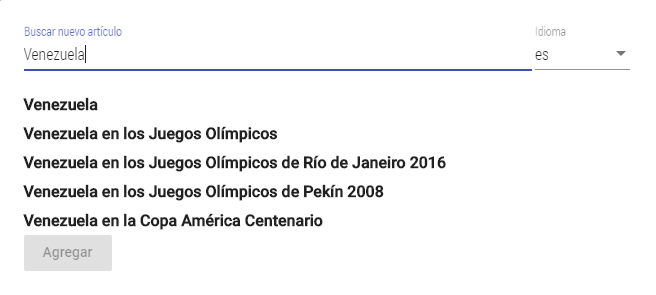
\includegraphics[scale=0.6]{images/marco_aplicativo/sugerencia_wikipedia.png}
      \captionof{figure}{Caja de sugerencias de artículos de Wikipedia}
      \label{fig:sugerencia_wikipedia}
      \bigbreak
  \end{center} 
  
  \item\textbf{Implementar componente y servicio para agregar artículo:}\\
  
  Surge la necesidad de persistir los artículos agregados por los usuarios, por lo que se tiene que habilitar la opción para crear artículos y extraerlo asíncronamente usando el API de Wikimetrics 2.0.
  
  Se abstrae el request a API para crear un artículo a través de un servicio, y se encapsula el componente de la tarea anterior en otro componente que interactué con el servicio.
  
  \begin{center}
      \bigbreak
      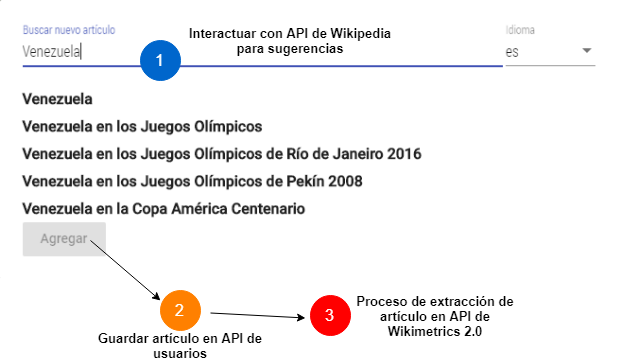
\includegraphics[scale=0.5]{images/marco_aplicativo/nuevo_articulo_flujo.png}
      \captionof{figure}{Flujo del agregar artículo, en el punto (1) se accede al api de Wikipedia para obtener los artículos sugeridos, luego al presionar agregar sucede el punto (2) que hace un request al API nuestra de usuarios para agregar el artículo y luego en el punto (3) se hace un request en el API de Wikimetrics 2.0 para activar el proceso de extracción del artículo}
      \label{fig:nuevo_articulo_flujo}
      \bigbreak
  \end{center} 
  
  \item\textbf{Implementar servicio para obtener lista de artículos:}\\
  
  Hasta ahora se había trabajado con una lista de artículos falsa desde una variable, donde entra la necesidad de poder pedir la lista de artículos asociada a un usuario.
 
  Se elabora el request a la ruta para pedir los artículos encapsulada en un servicio.

  \item\textbf{Crear componente dedicado a la carta de artículos:}\\
  
  El estilo de los artículos en el listado es hasta ahora muy simple y vacío.
 
  Se encapsula la lógica de la carta de un artículo en un componente, para abstraer funcionalidades complejas y se muestra más información del mismo, con un mejor estilo.

  \item\textbf{Actualizar estado del artículo cada cierto tiempo:}\\
  
  Sabemos que tenemos hacer un proceso de extracción del artículo para que el API de Wikimetrics pueda ofrecernos luego datos a visualizar de este, pero actualmente no tenemos forma se saber si el artículo ya fue extraído o no, de alguna forma tenemos que darle esa información al usuario para que esté al tanto del proceso. Un artículo puede tardar varios minutos en extraerse, todo esto depende del tamaño y cantidad de ediciones.
 
  Cuando un artículo es mandado a extraer, este responde con un código que nos servirá para preguntar por su estado. Replicamos esta lógica en el lado del API de usuarios, guardando el código y su estado actual:
  \begin{minted}[linenos]{json}
     {
        "locale": "es",
        "extract": {
            "status": "pending",
            "id": "665d387e-e547-4275-8abf-1076eacf8f92"
        },
        "title": "Universidad Central de Venezuela"
    }
  \end{minted}
  
  El proceso de extracción puede pasar por 4 estados: \textit{pending}, \textit{success}, \textit{failure}, \textit{in progress}.
  
  Para dar una interacción mas precisa al usuario, cada 10 segundos se hace un request para comprobar el estado y se actualiza en nuestra API, la condición de parada es que este \textit{success} o \textit{failure}
  
  \begin{center}
      \bigbreak
      
\includegraphics{images/marco_aplicativo/article_pending.png}
      \captionof{figure}{Estilo de un artículo en estado pendiente de extracción}
      \label{fig:article_pending}
      \bigbreak
  \end{center}
  \begin{center}
      \bigbreak
      
\includegraphics{images/marco_aplicativo/article_extracted.png}
      \captionof{figure}{Estilo de un artículo en estado exitoso de extracción}
      \label{fig:article_success}
      \bigbreak
  \end{center} 
  
  \item\textbf{Manejar autorización en las vistas:}\\
  
  Por lo momentos no hay ningún método que proteja las vistas que requieran autenticación, es decir anteriormente podemos intentar acceder a la vista del listado de artículos sin haber iniciado sesión, queda claro que al entrar a esta vista la petición daría error por seguridad del API.
  
  Agregamos una capa más de seguridad a nivel de cliente, para que el usuario no puede entrar sin autenticación a dichas vistas. Para esto usaremos guardias de rutas, a continuación la definición del guardia:
  \begin{minted}[linenos]{ts}
    import { Injectable } from '@angular/core';
    import { CanActivate, Router } from '@angular/router';
    import { AuthService } from './auth.service';
    
    @Injectable()
    export class AuthGuard implements CanActivate {
    
      constructor(
        private authSvc: AuthService,
        private router: Router) {}
    
      canActivate() {
        if (!this.authSvc.isSigned()) {
          this.router.navigate(['/sign-in']);
        }
    
        return this.authSvc.isSigned();
      }
    }
  \end{minted}
  
  Podemos observar que antes de navegar a una ruta la función \textbf{canActivate()} se llamará, esto verifica si hay una sesión de usuario válida, en caso contrario redirige al inicio de sesión.

  \item\textbf{Implementar barra superior (navbar):}\\

  Es importante desplegar una barra superior que muestre información extra y despliegue acciones, principalmente navegación a vista principal y cerrar sesión.
  
  
  Se implementó un componente para la barra y un servicio para cambiar sus configuraciones, como título, acciones y cierre de sesión.
  
  \begin{center}
      \bigbreak
      
\includegraphics[scale=0.6]{images/marco_aplicativo/navbar.png}
      \captionof{figure}{Barra superior}
      \label{fig:navbar}
      \bigbreak
  \end{center} 
  
  \item\textbf{Implementar ruta en API para obtener un artículo en especifico:}\\

  Al entrar al detalle de un artículo necesitamos solicitar la información de ese artículo en particular.
  
  Implementamos en API la nueva ruta:
  \begin{minted}{console}
   GET /articles/<idioma>/tituto
  \end{minted}
  
  Luego la adaptamos al componente del detalle de artículo.
  
  \item\textbf{Implementar servicio para pedir información sobre revisiones de un artículo:}\\

  En el detalle de artículo mostraremos cierta información básica sobre las ediciones, como el número total de ediciones y las últimas 20.
  
  Para tener el número total de ediciones tenemos que hacer uso de una ruta que wikimetrics nos provee:
  
  \begin{minted}{console}
   GET /api/v1/count?locale=en&title=Venezuela
  \end{minted}
  
  Para tener la información de las últimas 20 ediciones ordenadas por fecha descendientemente:
  \begin{minted}{console}
   GET /api/v1/revisions?locale=en&title=Venezuela
   &page_size=20&sort=desc
  \end{minted}
  
  Se encapsularon en el servicio de wikimetrics para abstraer su uso.

  \item\textbf{Implementar componente de visualización:}\\

  Algo sumamente importante es la posibilidad de desplegar gráficas, en distintos casos, la aplicación necesitará de un componente que muestre gráficas variables.
  
  Se abstraerá la visualización de un gráfica en un componente, apoyándonos de la biblioteca de Plotly. El componente acepta las siguientes entradas para variar su configuración:
  
  \begin{minted}[linenos]{ts}
  @Input() chartType: 'pie' | 'bar' | 'scatter'
    | 'scattergl' | 'line' | 'area';
  @Input() chartX: string[] | number[];
  @Input() chartY: string[] | number[];
  @Input() chartXTitle = '';
  @Input() chartYTitle = '';
  @Input() chartTitle = '';
  \end{minted}
  
  En donde \textbf{chartType} es para pasarle el tipo de gráfica que queremos desplegar, \textbf{chartX} y \textbf{chartY} correponde el set de datos para ambos ejes, \textbf{chartXTitle} y \textbf{chartYTitle} describe el título de ambos ejes y \textbf{chartTitle} hace referencia al título de la visualización.
  
  
  Se consideró hacer el componente de tal forma que fuera reactivo al cambio dimensión de la pantalla, es decir, las visualizaciones son responsive.
  
  \begin{minted}[linenos]{ts}
  this.resizeService.onResize$.subscribe(() =>
    Plotly.Plots.resize(this.gd)
  );
  \end{minted}
  
  Haciendo uso del patrón observador, con ayuda de la biblioteca ReactiveX \footnote{\url{http://reactivex.io/}}, cada ves que la pantalla cambia su posición nos enteramos mediante un servicio y ajustamos el tamaño de la visualización.
  
  \item\textbf{Mostrar información especifica en el detalle del artículo:}\\

  Al entrar al detalle del artículo nos tenemos que encontrar con información específica y que sume valor.
  
  Por lo tanto, consideramos colocar el número de ediciones, fecha de última edición, autor de la última edición, tamaño del artículo y una visualización que considere el tamaño y fecha de las ultimas 20 ediciones.
  
  \begin{center}
      \bigbreak
      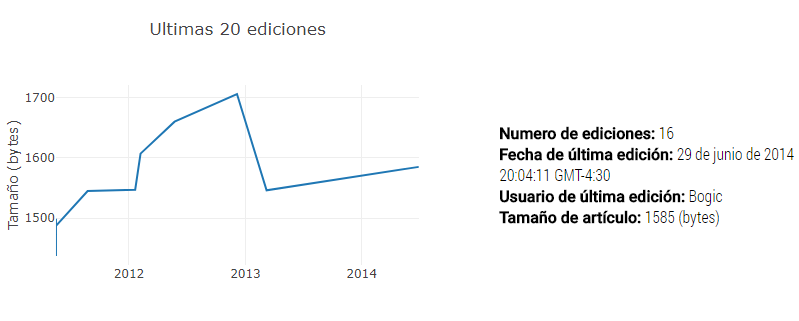
\includegraphics[scale=0.5]{images/marco_aplicativo/article_detail_main.png}
      \captionof{figure}{Visualización e información específica del artículo}
      \label{fig:article_detail_main}
      \bigbreak
  \end{center}
  
  De la siguiente manera quedaría el código para mostrar la gráfica, haciendo uso del componente de visualización :
  \begin{minted}[linenos]{html}
  <app-visualization
    chartTitle="Ultimas 20 ediciones"
    chartYTitle="Tamaño (bytes)"
    chartType="scatter"
    [chartX]="timestamps(revisions)"
    [chartY]="sizes(revisions)" 
    fxFlex="60" fxLayout="column">
  </app-visualization>
  \end{minted}
  
  Las función \textbf{timestamps(revisions)} extrae la fecha de edición y la función \textbf{sizes(revisions)} extrae el tamaño de cada edición
  
  
  \item\textbf{Implementar gráfica WikiHistoryFlow:}\\

  A nivel de visualizaciones, ofrecer la gráfica WikiHistoryFlow era un requerimiento principal. Con esta gráfica podemos identificar el comportamiento de un usuario, el estado del artículo en el tiempo y detectar patrones de vandalismo.
  
  La visualización proviene principalmente de la herramienta de History Flow Visualization \cite{HistoryFlow}, que consta de barras laterales, donde cada barra representa una edición. La altura de la barra representa el tamaño, el color representa un usuario único y el ancho representa la distancia del texto del artículo de la versión anterior y la actual.
  
  \begin{center}
      \bigbreak
      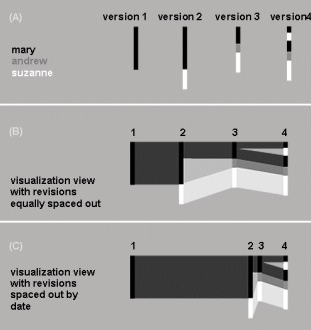
\includegraphics{images/marco_aplicativo/history_flow1.png}
      \captionof{figure}{Explicación del mecanismo usado en la visualización de History Flow}
      \label{fig:history_flow}
      \bigbreak
  \end{center}
  
  \begin{center}
      \bigbreak
      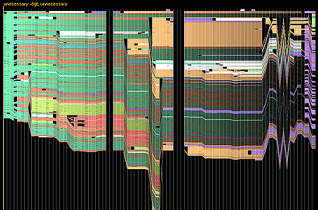
\includegraphics{images/marco_aplicativo/history_flow_original.png}
      \captionof{figure}{Herramienta History Flow Visualization}
      \label{fig:history_flow_original}
      \bigbreak
  \end{center}
  
  Para este trabajo por motivos de cómputos, se adaptara la visualización a una versión más simple, llamada History Graph \cite{HistoryGraph}.
  
  \begin{center}
      \bigbreak
      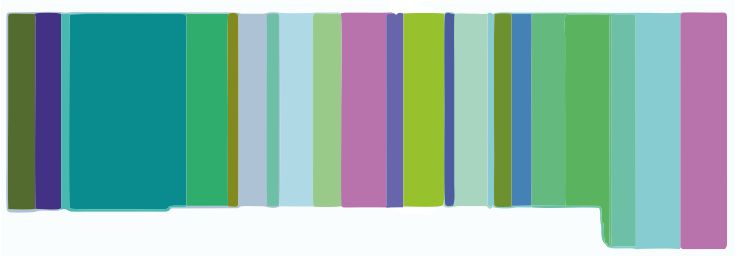
\includegraphics{images/marco_aplicativo/history_graph.png}
      \captionof{figure}{Visualización History Graph}
      \label{fig:history_graph}
      \bigbreak
  \end{center}
  
  No hay manera de desplegar esta gráfica con la biblioteca Plotly dado que es bastante específica, por lo tanto para este caso se optó por la biblioteca D3 que nos permite libertad a la hora de construir visualizaciones.
  
  Se encapsuló la visualización en un componente, en donde la primera tarea fue ordenar las ediciones por orden de creación de manera cronológica, luego se almacenó el valor de tamaño de edición máximo y se declaro un arreglo que contiene la distancia de cada edición contra la anterior (se asigno 0 para la primera edición). Para calcular la distancia entre dos textos se usó una biblioteca que aplica la distancia de Levenshtein.
  
  Calculados los datos anteriores tenemos todo listo para graficar, en donde cada elemento del arreglo de revisiones ordenado cronológicamente representa una barra usando el elemento \textbf{div} de html.
  
  \begin{minted}[linenos]{ts}
    d3.select(this.elemRef.nativeElement)
    .selectAll('div.bar')
    .data(revsOrderByDate)
    .enter().append('div').attr('class', 'bar')
  \end{minted} 
  
  Para asignar el ancho, se usó del arreglo de distancias antes calculado. Adicionalmente, se tiene que conservar el tamaño de manera proporcional a la pantalla, por lo que se le asigno a cada barra un ancho base predeterminado. Para que no ocurrieran desbordamiento de píxeles se uso una función de css llamada \textbf{calc} para ajustar el ancho base mas la distancia.
  
  \begin{minted}[linenos]{ts}
   .style('width', (_, i) => `calc(
    ${((1 / totalRev) * 100)}% + ${distanceRevs[i]}px
    )`
   )
  \end{minted} 
  
  Para asignar el alto basta con dividir el tamaño de la edición entre el tamaño máximo anteriormente calculado.
  
  \begin{minted}[linenos]{ts}
   .style('height', rev => `${(rev.size / maxSize) * 100}%`)
  \end{minted} 
  
  Finalmente, para asignar el color de la barra se usó una función hash que recibe un nombre de usuario (string) y retorna un color hexadecimal.
 
  \begin{minted}[linenos]{ts}
  .style('background', rev => 
    `${this.stringToColour(rev.user)}`
    )
  \end{minted}
  \begin{minted}[linenos]{ts}
  stringToColour(str: string) {
    let hash = 0;
    for (let i = 0; i < str.length; i ++) {
      // tslint:disable-next-line:no-bitwise
      hash = str.charCodeAt(i) + ((hash << 5) - hash);
    }
    let colour = '#';
    for (let i = 0; i < 3; i ++) {
      // tslint:disable-next-line:no-bitwise
      const value = (hash >> (i * 8)) & 0xFF;
      colour += ('00' + value.toString(16)).substr(-2);
    }
    return colour;
  }
  \end{minted} 
  
  Como funcionalidad adicional, se agregó un tooltip que muestra nombre del usuario, fecha y tamaño de la edición cuando nos apoyamos sobre cualquier barra.
  
  \begin{center}
      \bigbreak
      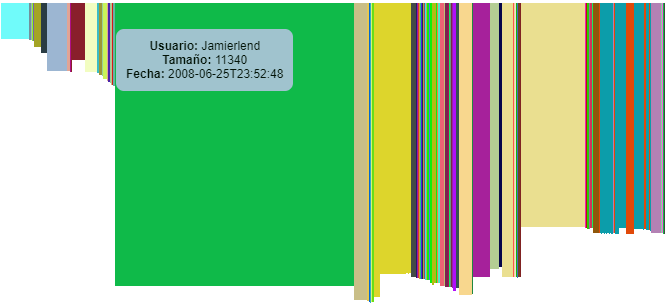
\includegraphics[scale=0.6]{images/marco_aplicativo/wiki_history_flow.png}
      \captionof{figure}{Visualización Wiki History Flow del artículo 'Programación dirigida por eventos'}
      \label{fig:wiki_history_flow}
      \bigbreak
  \end{center}
  
  
  
  \item\textbf{Agregar enlace a wikipedia del artículo:}\\

  En el detalle del artículo pude ser de gran utilidad tener un enlace que nos dirija al artículo en Wikipedia.
  
  \begin{center}
      \bigbreak
      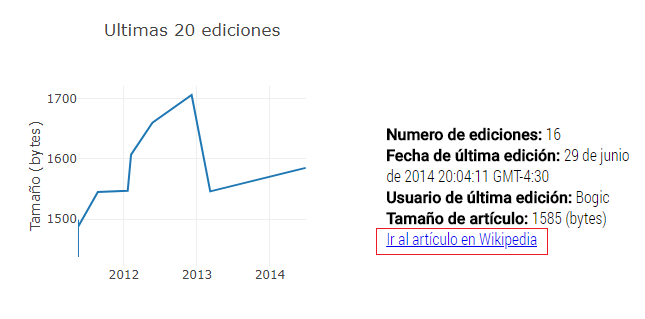
\includegraphics[scale=0.6]{images/marco_aplicativo/article_detail_main_with_link.png}
      \captionof{figure}{Información principal de detalle de artículo incluyendo vínculo a Wikipedia}
      \label{fig:article_detail_link}
      \bigbreak
  \end{center}
  
  \item\textbf{Implementar componente y servicio para crear nueva visualización:}\\

  Un requerimiento principal es poder crear nuestras visualizaciones sobre un artículo y poder editarlas, pero como primer paso necesitamos la creación de la misma preguntando información básica.
  
 
  Se posicionó un botón en el navbar capaz de crear la visualización. Al pisarlo mostrará un dialogo preguntando el título y descripción que tendrá la visualización.

  \begin{center}
      \bigbreak
      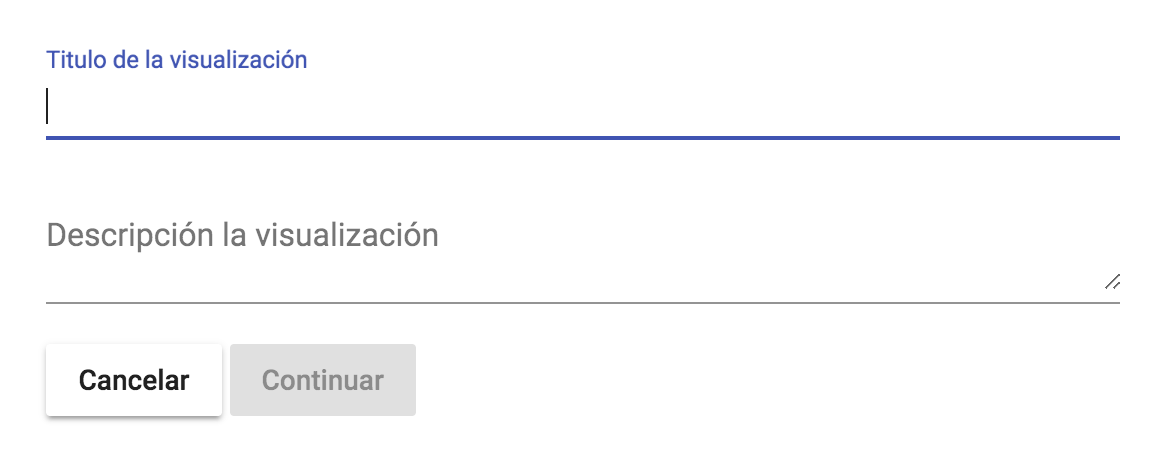
\includegraphics[scale=0.55]{images/marco_aplicativo/create_vis_main.png}
      \captionof{figure}{Información principal para crear una visualización}
      \label{fig:create_vis_main}
      \bigbreak
  \end{center}
  
  Dado esto, se manejó en base de datos un objeto de Visualizaciones donde la llave de cada atributo representa el título:

  \begin{minted}[linenos]{json}
   {
    "title": "Universidad Central de Venezuela",
    "visualizations": {
        "Visualización de usuarios": {
            "query": "",
            "type": "",
            "description": "Torta"
        },
        "Visualización de ediciones menores": {
            "query": "",
            "type": "",
            "description": ""
        }
    }
   }
  \end{minted}

  \item\textbf{Implementar componente y servicio para crear nueva visualización:}\\

  Es necesario listar las visualizaciones creadas en el detalle de artículo, para luego ser accedidas.
 
  Se crearon dos listas, una de las visualizaciones creadas por el usuario y otra de visualizaciones predefinidas por la aplicación.
 
  \item\textbf{Implementar componente para seleccionar el query de la visualización:}\\

  Creada una visualización es necesario empezar a editarla para construir la gráfica respectiva, por lo que necesitamos ofrecer la herramienta para seleccionar lo que se desear visualizar.
  
  La herramienta constará de tres (3) selectores, el primero permite filtrar, el segundo ofrece operaciones de agrupaciones y el tercero permite agrupar.
  
  El selector de \textbf{filtro} ofrece filtrar por edición anónima, tamaño de la edición, id de usuario, nombre de usuario, edición menor y fecha de edición.
  
  El selector de \textbf{vista} ofrece operadores sobre agrupaciones como contar, sumar tamaño de ediciones, promediar tamaño de ediciones, máximo tamaño de ediciones y mínimo tamaño de ediciones.
  
  El selector de \textbf{agrupar} ofrece la posibilidad de agrupar por edición anónima, id de edición, tamaño de edición, id de usuario, nombre de usuario, edición menor, fecha (mes), fecha (mes y año), fecha (día, mes y año).
  
  
  \begin{center}
      \bigbreak
      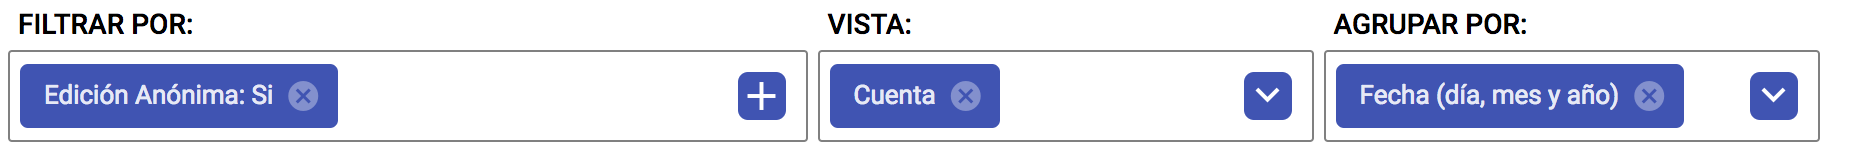
\includegraphics[scale=0.3]{images/marco_aplicativo/query_selector.png}
      \captionof{figure}{Vista de componente para seleccionar query de la visualización}
      \label{fig:query_selector}
      \bigbreak
  \end{center}
  
  El valor de cada opción de los selectores referencia a parte del query de mongodb necesario. Por lo tanto se realizó una función para construir el query final a enviar al API de Wikimetrics:
  
  \begin{minted}[linenos]{ts}
  buildQuery(): WikimetricsQuery[] {
    // setup filters
    let obj = {};
    this.selectedFilters.forEach(i => {
      obj = merge(obj, i.value);
    });

    // build query
    const newQuery = [
      {
        $match: obj
      },
      {
        $group: {
          _id: this.selectedGroup ?
          this.selectedGroup.value : null ,
          ... this.selectedView && this.selectedView.value ?
          { result: this.selectedView.value } : {}
        }
      }
    ];

    return newQuery;
  }
  \end{minted}
  
  En donde \textbf{obj} es el objeto con todos los filtros, \textbf{selectedGroup.value} el campo u objeto de la agrupación y \textbf{selectedView.value} el nombre del operador de agrupaciones.
  
  Por último, si ya tenemos un query formado, necesitamos la función inversa que sería extraer del query los valores para rellenar los selectores. Esta funcionalidad es extensa por lo que se puede revisar en el código fuente del proyecto en el componente \textbf{query-selector.component.ts}.
  
  \item\textbf{Implementar componente para editar visualizaciones:}\\

  Cuando obtenemos la respuesta del query, tenemos los datos pero no listos para visualizarlos, tenemos que darle un formato entendible para usarlo con el componente de visualización anteriormente creado, además tenemos que definir el tipo de visualización a mostrar.
  
  
  Se tuvo que condicionar cada uno de los casos posibles de las opciones, en el caso de edición menor, interpretar a 'No menor' y 'Menor', para usuario anónimo se interpretó como 'Anónimo' y 'No Anónimo'. En el caso de agrupación por fecha se usó la biblioteca luxon\footnote{\url{https://moment.github.io/luxon/}} (alternativa ligera de moment) para darle un mejor formato.
  
  
  \begin{center}
      \bigbreak
      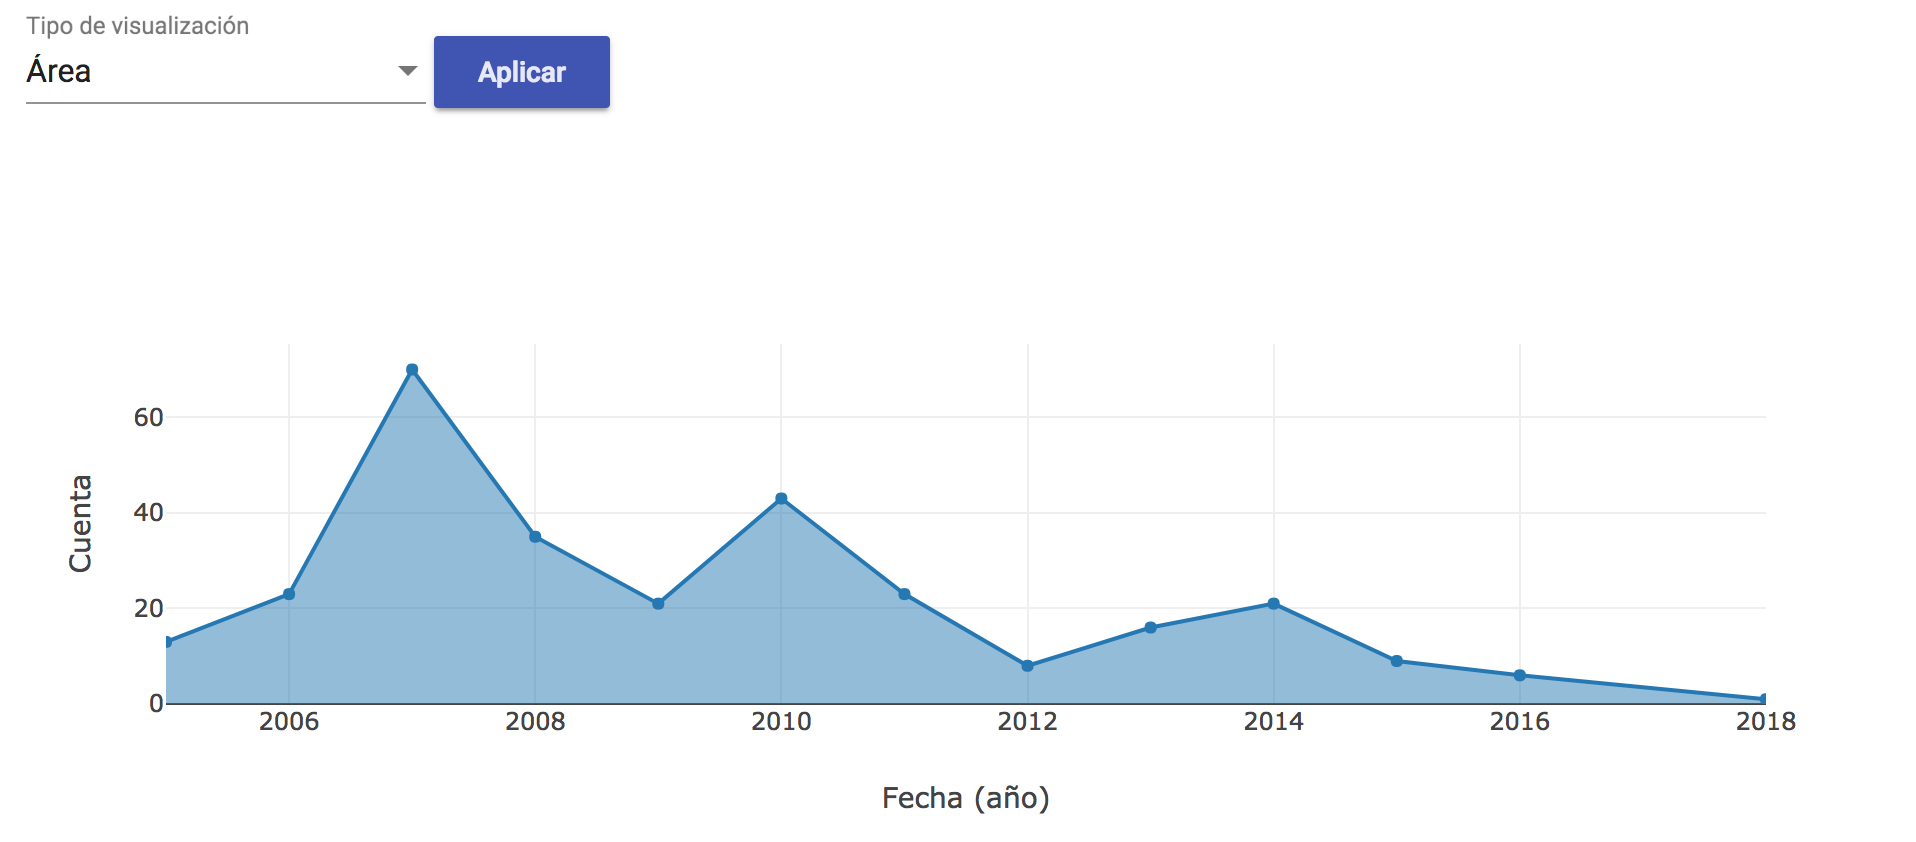
\includegraphics[scale=0.35]{images/marco_aplicativo/edit_vis.png}
      \captionof{figure}{Componente de visualización y selector de tipo en el editor de visualizaciones}
      \label{fig:edit_vis}
      \bigbreak
  \end{center}
  
  El selector de tipo visualizaciones ofrece los siguientes:
  \begin{itemize}
    \item\textbf{Número}: muestra un número total, solo es válido cuando no se aplica agrupación.
    
        \begin{center}
          \bigbreak
          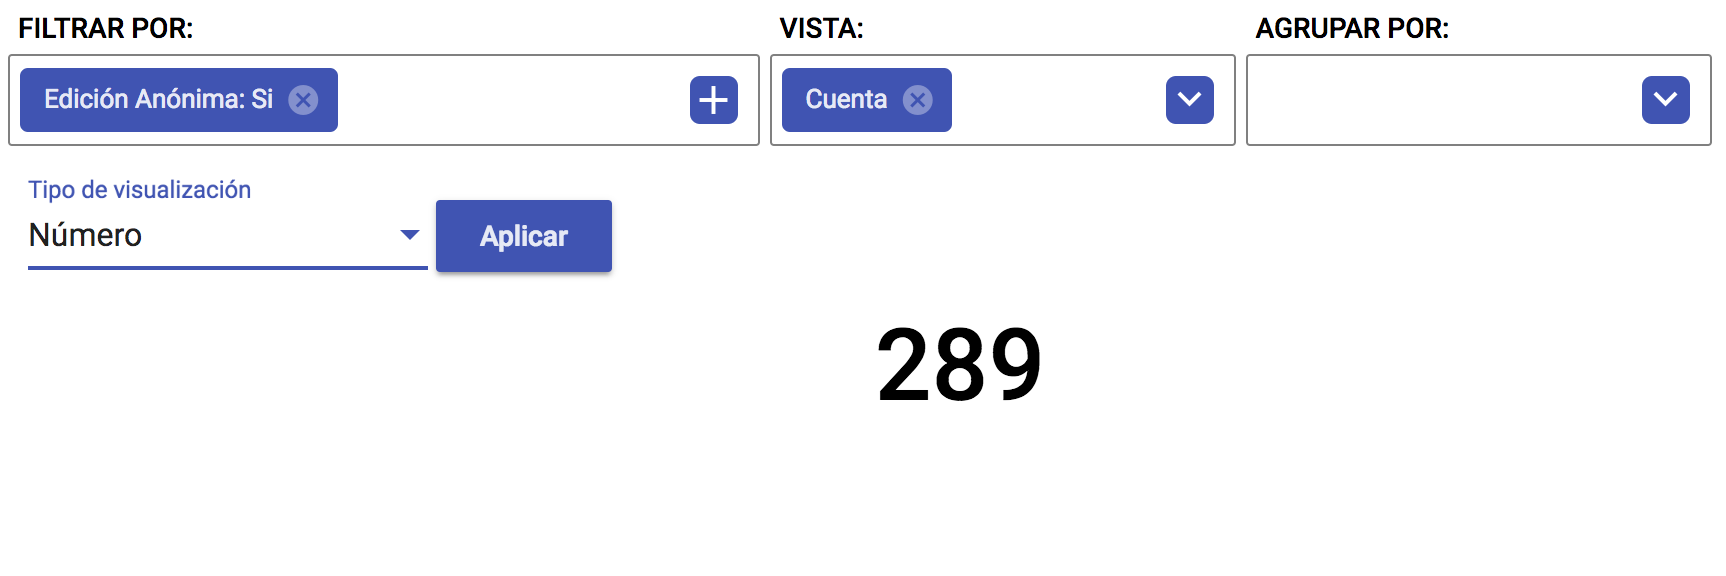
\includegraphics[scale=0.35]{images/marco_aplicativo/vis_number.png}
          \captionof{figure}{Visualización tipo número}
          \label{fig:vis_number}
          \bigbreak
        \end{center}

    \item\textbf{Línea}: gráfica que consiste en trazar un línea entre cada par de puntos.
        \begin{center}
          \bigbreak
          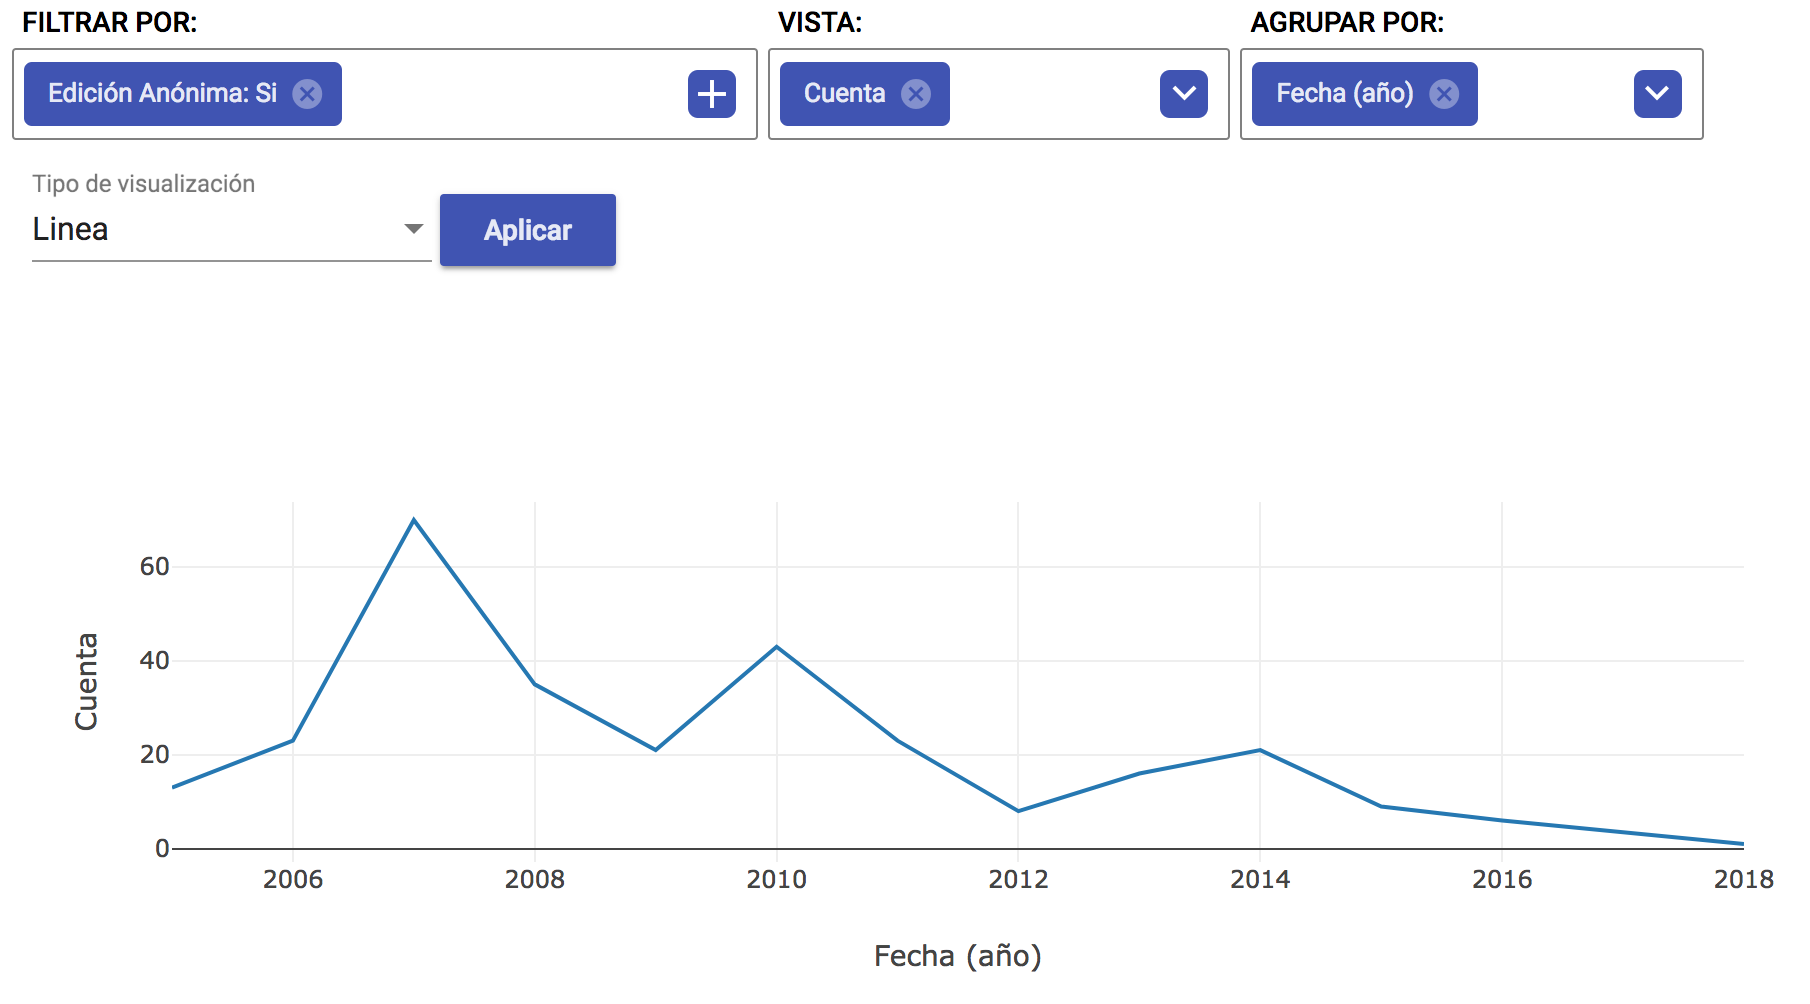
\includegraphics[scale=0.35]{images/marco_aplicativo/vis_line.png}
          \captionof{figure}{Visualización tipo línea}
          \label{fig:vis_line}
          \bigbreak
        \end{center}

    \item\textbf{Barra}: gráfica que consiste en proyectar barras.
        \begin{center}
          \bigbreak
          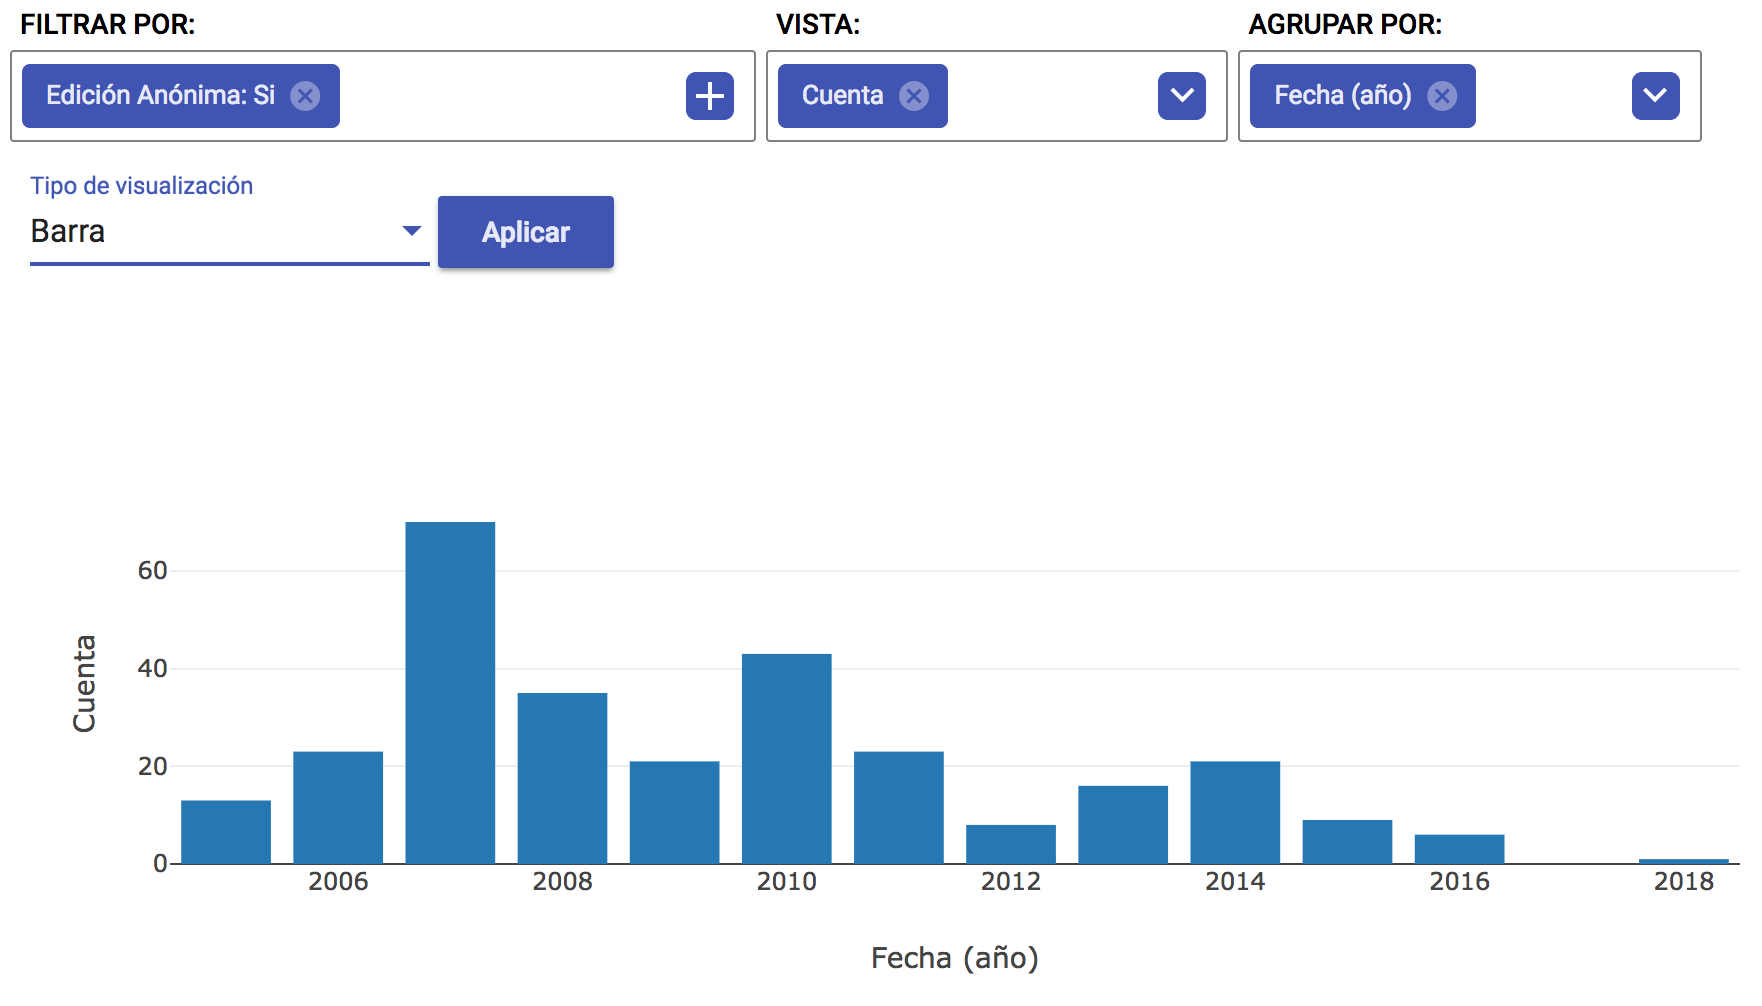
\includegraphics[scale=0.35]{images/marco_aplicativo/vis_bar.png}
          \captionof{figure}{Visualización tipo barra}
          \label{fig:vis_bar}
          \bigbreak
        \end{center}

    \item\textbf{Área}: gráfica similar a la de línea pero con el área pintada. Se puede observar en la \textbf{Figura \ref{fig:edit_vis}}.
    
    \item\textbf{Torta}: gráfica circular en donde los datos son representados por proporción.
        \begin{center}
          \bigbreak
          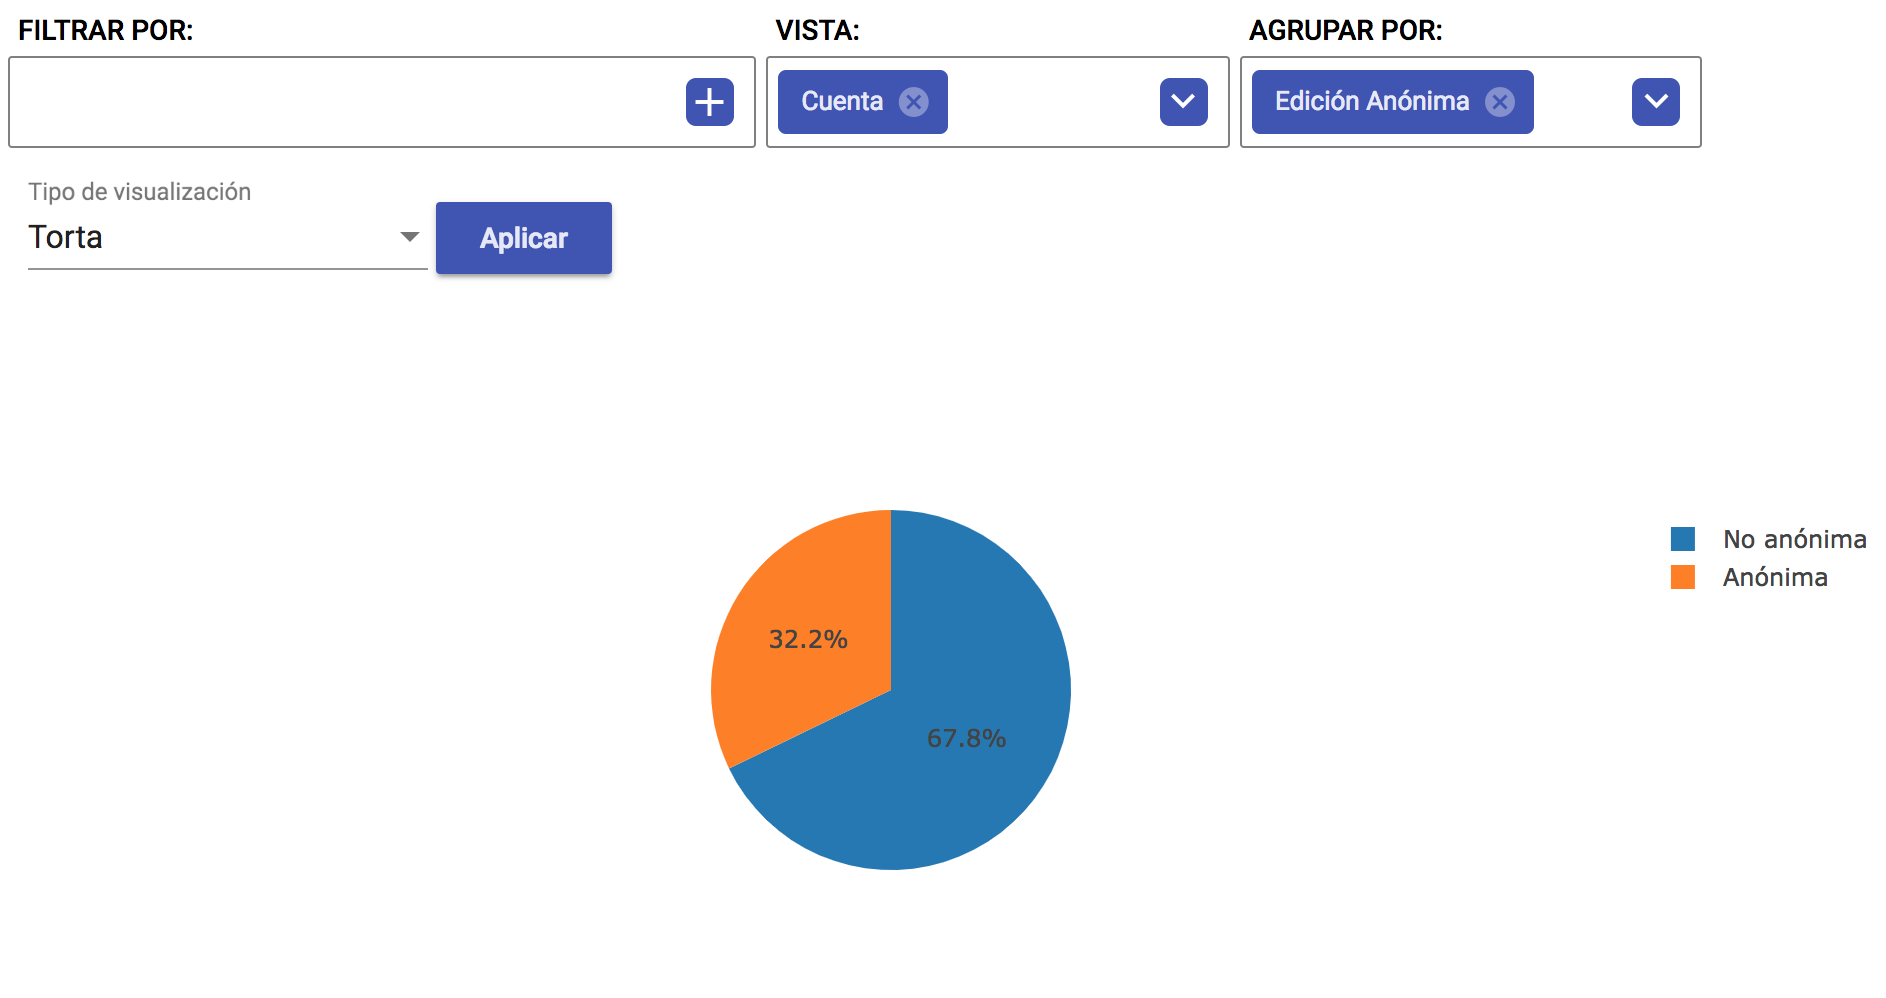
\includegraphics[scale=0.3]{images/marco_aplicativo/vis_pie.png}
          \captionof{figure}{Visualización tipo torta}
          \label{fig:vis_pie}
          \bigbreak
        \end{center}
        
    \item\textbf{Dispersión}: gráfica donde cada dato es representado por un punto.
        \begin{center}
          \bigbreak
          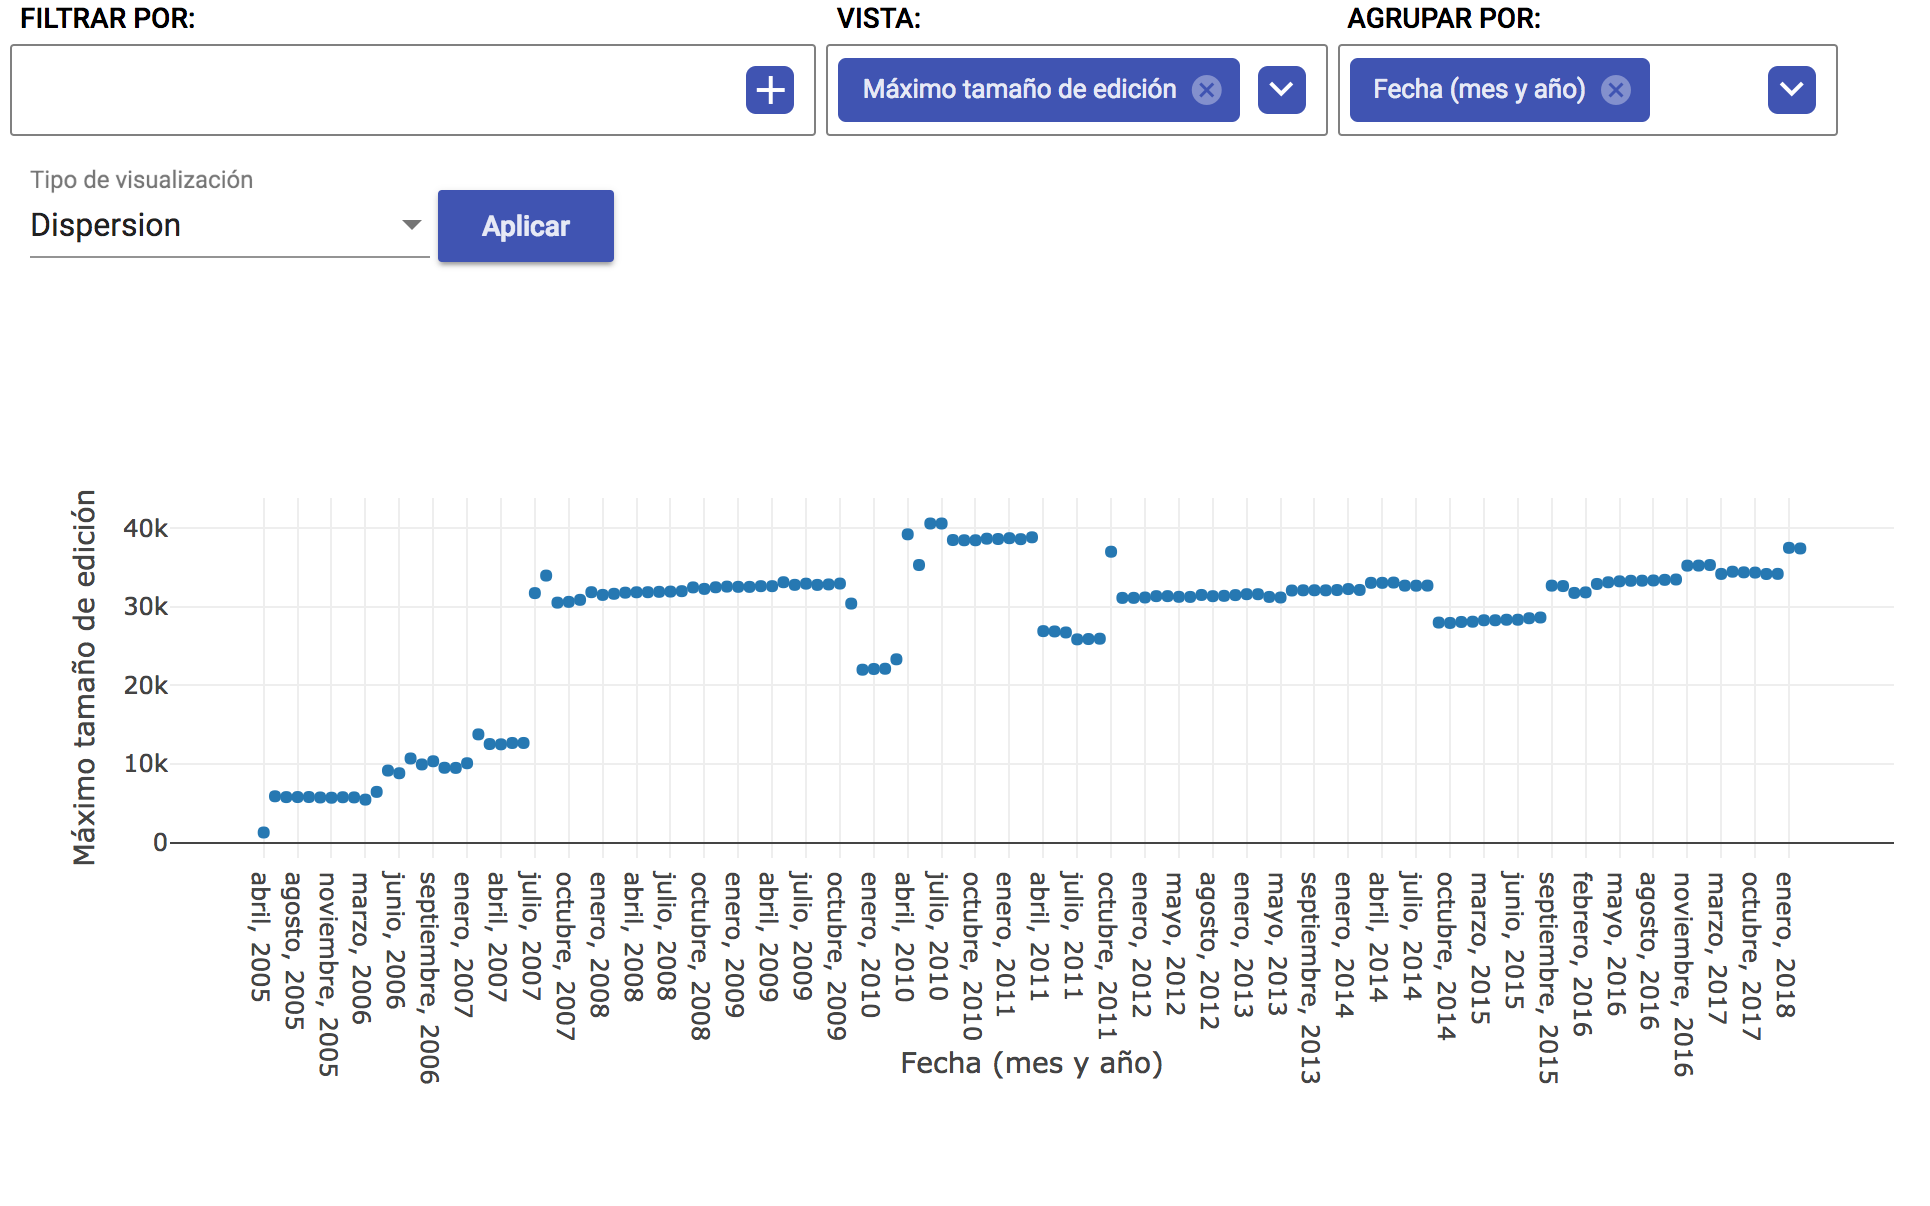
\includegraphics[scale=0.35]{images/marco_aplicativo/vis_scatter.png}
          \captionof{figure}{Visualización tipo dispersión}
          \label{fig:vis_scatter}
          \bigbreak
        \end{center}
  \end{itemize}
  
  \item\textbf{Implementar borrar artículo y visualización:}\\
  
  Hasta ahora podemos crear artículos y visualizaciones, pero no borrar.
  
  Se implementaron las rutas en el API usando el método DELETE de HTTP para ambos recursos, cada servicio, el de visualizaciones y artículos se encapsuló el request. Por último, se habilitó la acción de eliminar en la interfaz para ambos casos.
  
  \item\textbf{Agregar zoom a gráfica del editor de visualizaciones:}\\

  En el editor de visualizaciones puede que una visualización este tan cargada de datos que la información se resuma y no se muestre toda, por lo que no veremos todos los datos.
  
  
  Plotly, automáticamente esconde la información para no sobrecargar la visualización, pero nos provee la funcionalidad de navegar en la visualización haciendo zoom.
  
  \begin{minted}[linenos]{ts}
  const layout = {
    xaxis: { title: this.chartXTitle, fixedrange: !this.chartZoom},
    yaxis: { title: this.chartYTitle, fixedrange: true},
  };
  \end{minted}
  
  La biblioteca nos permite pasarle un objeto con configuraciones al graficar. El atributo \textbf{xasis} hace referencia al eje 'x' y el atributo \textbf{yasis} al eje 'y'. Habilitaremos el zoom en el eje 'x' solamente y lo manejaremos con un input llamado \textbf{chartZoom}.
  
  \item\textbf{Agregar filtro de fecha en gráfica de Wiki History Flow:}\\
  
  La gráfica Wiki History Flow suele ser muy pesada, en artículos con muchas ediciones puede tomarse un tiempo considerable en cargar debido a la petición de la información y el algoritmo para extraer la distancia del contenido.
  
  Como mecanismo para evitar larga espera, se implemento un filtro por rango de fecha, en donde se cargará solo las ediciones realizas en ese rango.
  
  En la primera carga se definió un rango de fecha que involucren las 200 primeras ediciones del artículo.

  \begin{center}
    \bigbreak
    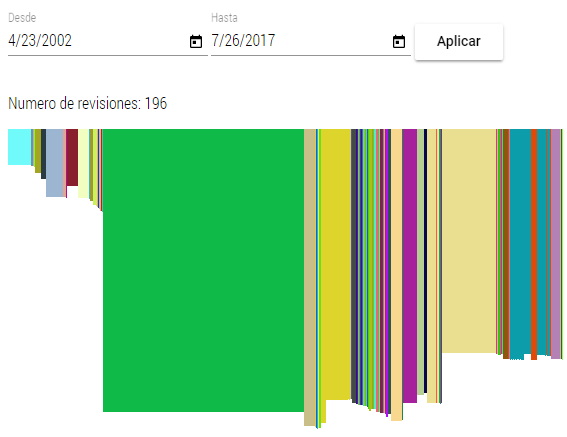
\includegraphics[scale=0.35]{images/marco_aplicativo/date_range_wiki_history_flow.png}
    \captionof{figure}{Wiki History Flow con filtro de rango de fecha.}
    \label{fig:date_range_wiki_history_flow}
    \bigbreak
  \end{center}
  
  
  \item\textbf{Agregar componente de preview de visualización:}\\

  Para poder observar una visualización es necesario entrar al detalle del artículo y seleccionar la que queremos editar en el listado. Surge la necesidad de observar la gráfica de la visualización sin necesidad de acceder al editor.
  
  
  Se implementó una propiedad llamada \textit{preview}, donde cada elemento de la lista de visualizaciones proveerá la acción de habilitar o no el preview de dicha visualización.
  
  \begin{center}
    \bigbreak
    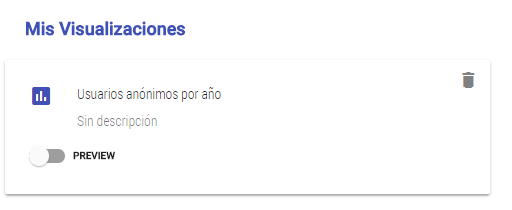
\includegraphics[scale=0.7]{images/marco_aplicativo/toggle_preview.png}
    \captionof{figure}{Toggle para habilitar/deshabilitar preview.}
    \label{fig:toggle_preview}
    \bigbreak
  \end{center}
  
  Al habilitar el preview la gráfica de la visualización será mostrada en una sección del detalle de actividad haciendo uso del componente de visualización.
  
  \begin{center}
    \bigbreak
    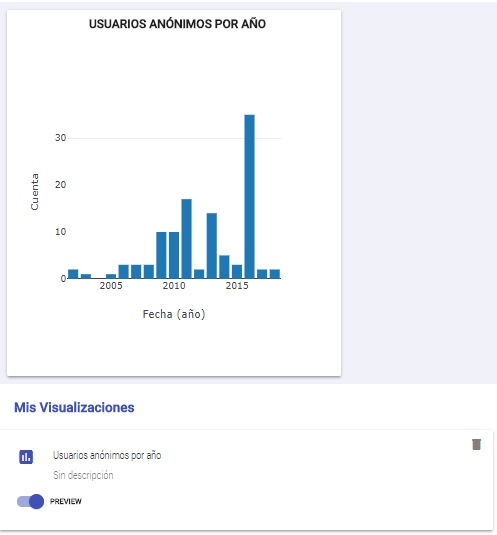
\includegraphics[scale=0.7]{images/marco_aplicativo/vis_preview.png}
    \captionof{figure}{Componente preview de visualización en detalle de artículo.}
    \label{fig:toggle_preview}
    \bigbreak
  \end{center}
  
  El preview puede ser pisado y nos dirige al editor de la misma.
  
  \item\textbf{Incluir número de ediciones menores (con porcentaje) y número de editores en detalle de artículo:}\\
  
  Se consideró agregar más información en el detalle del artículo, en donde el número de ediciones menores y número de editores pueden ser de utilidad.
  
  Apoyándonos de la flexibilidad del API, para obtener el número de ediciones del artículo enviamos el siguiente query:
  \begin{minted}[linenos]{json}
    [
      {
        "$match": {
          "title": "Programación dirigida por eventos",
          "locale": "es",
          "minor": {
            "$exists": true
          }
        }
      },
      {
        "$group": {
          "_id": null,
          "result": {
            "$sum": 1
          }
        }
      }
    ]
  \end{minted}
  
  Para obtener el número de editores enviamos el siguiente query y calculábamos el tamaño de la respuesta:
  \begin{minted}[linenos]{json}
    [
      {
        "$match": {
          "title": "Programación dirigida por eventos",
          "locale": "es"
        }
      },
      {
        "$group": {
          "_id": "$userid",
          "result": {
            "$sum": 1
          }
        }
      }
    ]
  \end{minted}

  \item\textbf{Definir e implementar gráficas generales en el detalle del artículo:}\\
  
  Existen ciertas visualizaciones que seguramente sean de interés, por lo que podemos ofrecerlas de manera predeterminada y evitar que el usuario pierda tiempo en la creación de las mismas.
  
  En la lista de visualizaciones predeterminadas, en el detalle del artículo, se agregaron las siguientes visualizaciones: Ediciones menores, Usuario anónimos, Top 10 editores y Número de ediciones por mes y año.
  
  La información de estas visualizaciones se encuentran de manera estática por ahora dentro del código.
  
  Se implementó un componente capaz de visualizarlas en una vista nueva, similar al preview y este fue el resultado:
  
  \begin{center}
    \bigbreak
    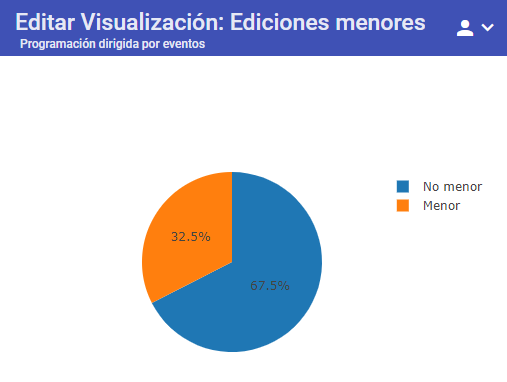
\includegraphics[scale=0.7]{images/marco_aplicativo/vis_default_minor_edit.png}
    \captionof{figure}{Visualización predefinida de total de ediciones menores vs. no menores del artículo 'Programación dirigida por eventos'}
    \bigbreak
  \end{center}
  
  \begin{center}
    \bigbreak
    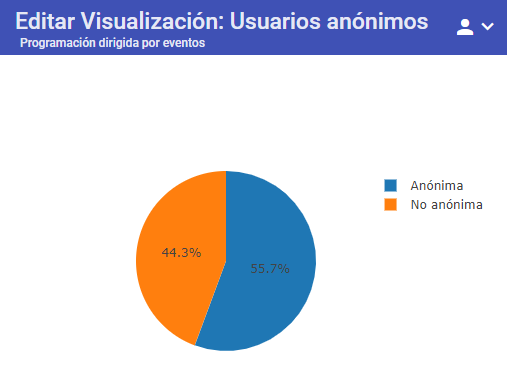
\includegraphics[scale=0.7]{images/marco_aplicativo/vis_default_anon_user.png}
    \captionof{figure}{Visualización predefinida de total de usuarios anónimos vs. no anónimos del artículo 'Programación dirigida por eventos'}
    \bigbreak
  \end{center}

  \begin{center}
    \bigbreak
    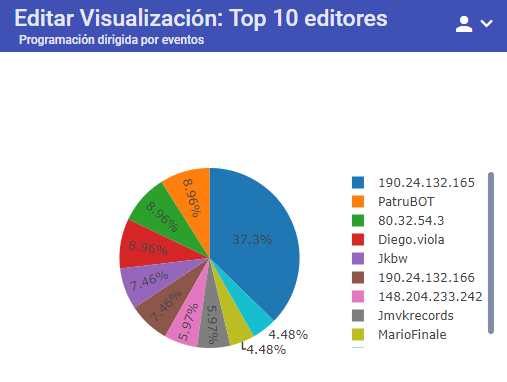
\includegraphics[scale=0.7]{images/marco_aplicativo/vis_default_top_10.png}
    \captionof{figure}{Visualización predefinida de Top 10 de usuarios con más ediciones del artículo 'Programación dirigida por eventos'}
    \bigbreak
  \end{center}

  \begin{center}
    \bigbreak
    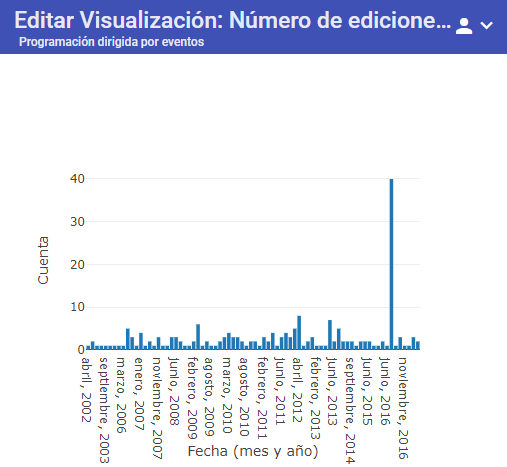
\includegraphics[scale=0.7]{images/marco_aplicativo/vis_default_count_month_year.png}
    \captionof{figure}{Visualización predefinida de total de ediciones agrupadas por mes y año del artículo 'Programación dirigida por eventos'}
    \bigbreak
  \end{center}
  
  

\end{enumerate}

% Conclusiones
\chapter{Conclusiones}
En el presente trabajo se analizó, diseñó e implementó una aplicación web capaz de ofrecer a un usuario una herramienta para gestionar visualizaciones sobre ediciones de un artículo wiki. Como primer requerimiento el usuario tiene que crearse una cuenta para mantener una sesión privada, luego podrá agregar artículos principalmente de Wikipedia en idioma Español e Inglés, esto requiere que se active el proceso de extracción en el API de Wikimetrics para obtener las ediciones del mismo. Una vez extraído el artículo podemos acceder al detalle en donde encontraremos información específica y base como número de ediciones, número de ediciones menores, fecha de ultima edición, usuario de ultima edición, número de usuarios que editaron, tamaño de artículo y link al artículo de Wikipedia. Esta vista de detalle ofrece también la posibilidad de crear visualizaciones y una lista donde se muestran. Además, se presentará una lista de visualizaciones predeterminadas, entre ellas la que resalta es la gráfica Wiki History Flow. Las visualizaciones creadas por el usuario pueden habilitarse para mostrar su preview en una sección del mismo detalle de artículo, al presionar tanto el preview como la visualización del listado podemos entrar al editor de visualizaciones. En el editor de visualizaciones se nos presenta un selector en donde podemos definir el filtro, la vista y la agrupación, luego de esto tenemos un selector para definir el tipo de gráfica a visualizar. 

Para la construcción de la aplicación nos apoyamos del framework Angular y Angular Material para el diseño, fue necesario usar el API de Wikipedia para ofrecer las sugerencias de artículos en la creación del mismo. Para las visualizaciones extraemos los datos del API de Wikimetrics y nos apoyamos de las bibliotecas D3 y Plotly para graficarlas de manera fácil.

\begin{center}
    \bigbreak
    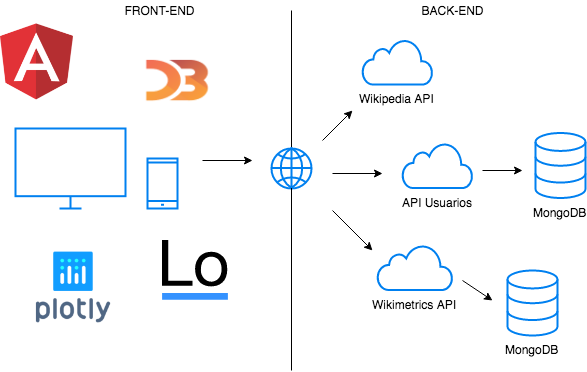
\includegraphics[scale=0.45]{images/conclusiones/tech_context.png}
    \captionof{figure}{Esquema abstracto de las tecnologías involucradas en el trabajo}
    \label{fig:library_comparison}
    \bigbreak
\end{center}


\section{Contribuciones}
\begin{itemize}
    \item Se realizó una investigación amplia de bibliotecas de visualización que puede servir como apoyo para la decisión de futuros trabajos dependiendo de los requerimientos.
    
    \item Se realizó investigación en el área de Visualización de Datos, refrescando conceptos teóricos claves y planteamientos de como resolver problemas haciendo uso de diferentes técnicas.
    
    \item Se implementó un componente en Angular que facilita la creación de visualizaciones responsives usando Plotly, en donde será de apoyo para aquellos trabajos que involucren las mismas tecnologías.
    
    \item Se elaboró un componente de Angular que construye la gráfica Wiki History Flow haciendo uso de D3. Para trabajos futuros puede servir de apoyo para la mejora o construcción de la misma.
    
    \item Al ser una aplicación web que implica tecnologías nuevas e interesantes puede aportar contenido y ejemplos para la materia de Aplicaciones en Internet.
\end{itemize}

\section{Limitaciones}

\begin{itemize}
    \item Principalmente se iba a usar el API de Wikipedia para realizar la autenticación de usuarios y extraer los artículos de su watchlist como primera instancia, pero Wikipedia dejó obsoleta la manera vieja de autenticación y la nueva forma es mediante OAuth2, por lo que pedían usa serie de requerimientos que estaban fuera del alcance. Por tal motivo se optó por gestionar los usuarios con nuestro propio sistema.
    
    \item Para la realización de visualizaciones se tuvo que diseñar e implementar un nuevo end-point en el API de Wikimetrics debido a que los otros eran pocos flexibles. Por lo tanto se tomó tiempo del trabajo para el análisis de la misma. Con el nuevo end-point por falta de tiempo los queries en mongo los tuvo que definir el front-end en base a los requerimientos.
\end{itemize}

\section{Trabajos futuros}

\begin{itemize}
    \item Dejar de manejar los usuarios internamente y manejar la autenticación con el API de Wikipedia. Lo principal sería cumplir con los requerimientos que pide MediaWiki como API para crear la aplicación usando OAuth2. De esta forma solo manejaremos un inicio de sesión usando el usuario de Wikipedia.
    
    \item Habilitar una opción para poder sincronizar los artículos del watchlist del usuario de Wikipedia con los artículos de esta plataforma.
    
    \item Analizar qué visualizaciones pueden ser frecuentes en los usuarios y ofrecerlas como visualizaciones predeterminadas.
    
    \item Implementar la gráfica original de History Flow. Esta visualización requiere de mucho cómputo, por lo que calcularlas en el front-end es inviable. La idea es delegarle esta funcionalidad a un servicio en el back-end que envíe los datos preparados para la visualización.
    
    \item Alguna funcionalidad para compartir dashboard de visualizaciones o visualizaciones individuales en modo de solo lectura
\end{itemize}

\clearpage

\addcontentsline{toc}{chapter}{Bibliografía}
\printbibliography
\end{document}
